%
% Niniejszy plik stanowi przykład formatowania pracy magisterskiej na
% Wydziale MIM UW.  Szkielet użytych poleceń można wykorzystywać do
% woli, np. formatujac wlasna prace.
%
% Zawartosc merytoryczna stanowi oryginalne osiagniecie
% naukowosciowe Marcina Wolinskiego.  Wszelkie prawa zastrzeżone.
%
% Copyright (c) 2001 by Marcin Woliński <M.Wolinski@gust.org.pl>
% Poprawki spowodowane zmianami przepisów - Marcin Szczuka, 1.10.2004
% Poprawki spowodowane zmianami przepisow i~ujednolicenie
% - Seweryn Karłowicz, 05.05.2006

\documentclass[licencjacka]{pracamgr}

\usepackage{polski}

\usepackage[utf8]{inputenc}

\usepackage{pdfpages}

\usepackage{gensymb}

\usepackage{url}

% Dane licencjanta:

\author	{Imię Nazwisko}

\nralbumu{666999}

\title{Implementacja taktycznej gry fabularnej czasu rzeczywistego}

\tytulang{An implementation of a real-time strategy role-playing game}

\kierunek{Informatyka}

\opiekun{mgra Radosława Bartosiaka\\
  Instytut Informatyki\\
  }

% miesiąc i~rok:
\date{Czerwiec 2015}

\dziedzina{11.3 Informatyka}

%Klasyfikacja tematyczna wedlug ACM (informatyka)
\klasyfikacja{D. Software}

\keywords{gra, gra komputerowa, qt, sfml, box2d, taktyczna gra fabularna}

% Tu jest dobre miejsce na~Twoje własne makra i~środowiska:
% \newtheorem{defi}{Definicja}[section]

% koniec definicji

\begin{document}
\maketitle

%tu idzie streszczenie na~strone poczatkowa
\begin{abstract}
  Niniejsza praca stanowi raport z~naszej pracy nad~taktyczną grą fabularną \emph{Buried Secrets} stworzoną w~ramach przedmiotu Zespołowy Projekt
  Programistyczny. Opisujemy w~niej założenia projektowe wraz~z~objaśnieniem silnika gry. Ponadto opisujemy architekturę 
  powstałego programu oraz~narzędzia i~metodologie wykorzystane przy pracy.
\end{abstract}

\tableofcontents
%\listoffigures
%\listoftables

\chapter*{Wprowadzenie}
\addcontentsline{toc}{chapter}{Wprowadzenie}
  Cyfrowa rewolucja, dziejąca się od~kilkudziesięciu lat, zmieniła niemal każdy aspekt życia współczesnego człowieka.
  Jedną z~tych zmian było spojrzenie na~komputer jako~potencjalne źródło rozrywki. Współcześnie, przemysł
  gier komputerowych, którego wartość szacuje się na~ok. 75 miliardów dolarów\cite{CA}, wciąż zyskuje na~popularności.
  Pomimo setek tysięcy wyprodukowanych gier, zaangażowania wielkich koncernów, wciąż istnieje na~rynku zapotrzebowanie
  na~nowe, oryginalne produkcje, które dostarczą graczowi niezapomnianych przeżyć i~przykują go~do~komputera na~długie godziny.

  Z~punktu widzenia twórcy, gry komputerowe stanowią jednak niezwykle trudne wyzwanie. Po~pierwsze, należy stawić czoła
  nieprzeciętnym problemom technicznym, wymagającym wszechstronnej wiedzy informatycznej, pozwalającej do maksimum wykorzystać
  dostępne medium. Po drugie, gry wymagają szerokiej wiedzy z~przeróżnych dziedzin, związanych
  z~grafiką, dźwiękiem, tworzeniem fabuły. W~końcu, należy te wszystkie składniki połączyć, mając przed sobą ostateczny cel: dostarczenie
  graczowi wysokiej jakości rozrywki. Skomplikowanie i~trudność w~sprecyzowaniu tego celu powodują, że~proces tworzenia gier
  znacząco różni się od~produkcji innego rodzaju oprogramowania. Dopiero harmonijne zgranie wszystkich składników, podporządkowanie
  ich spójnej wizji, ma szansę wywołać u~gracza niezapomniane przeżycia i~zapewnić twórcy pełną satysfakcję z~wykonanej pracy.

  Poniższa praca opisuje projekt realizowany przez nas w~ramach przedmiotu Zespołowy Projekt Programistyczny dla~Koła Programowania
  Gier Komputerowych działającego na~wydziale Matematyki, Informatyki i~Mechaniki Uniwersytetu Warszawskiego.
  Projekt ten dotyczył stworzenia silnika gry komputerowej, wraz z~przykładową implementacją gry. Stworzona gra nosi nazwę
  \emph{Buried Secrets}. W~kolejnych rozdziałach prezentujemy główne ograniczenia projektowe, opis założonego produktu końcowego,
  techniczne aspekty realizacji projektu, uzyskane rezultaty i~wnioski z~naszej rocznej pracy.


\chapter{Słownik}
  \paragraph{Content gry} ogólne określenie na~wszelkie elementy gry, niebędące częścią programu. Zwykle do~contentu zalicza się
    dźwięk, grafikę, wyświetlane teksty, parametryzację gry.
  \paragraph{Playtesty} część procesu tworzenia gry, podczas którego gra jest testowana w~poszukiwaniu błędów, wad projektowych mechaniki
    lub~interfejsu zanim trafi na~rynek.
  \paragraph{Poziom gry} logiczny fragment gry wyznaczony przez misję fabularną do~wykonania i~mapę odpowiedniej lokacji.
  \paragraph{Silnik gry} system informatyczny udostępniający gotowe funkcjonalności, potrzebne do~implementacji gry komputerowej.

\chapter{Projekt}

  \section{Opis projektu}
    Zgodnie z~zamówieniem klienta, realizowany projekt dotyczył stworzenia gry komputerowej
    średnich rozmiarów. Ze względu na~skład zespołu, złożonego wyłącznie z~programistów, skupiliśmy się
    na~dostarczeniu rozbudowanego, w~pełni funkcjonalnego silnika gry.
    Docelowa aplikacja miała być grywalnym produktem, prezentującym możliwości zaimplementowanego silnika,
    bez~contentu i~grafiki na~poziomie konkurencyjnych, komercyjnych gier. Dodatkowym wymogiem było zrealizowanie
    projektu, w~sposób umożliwiający dystrybucję na~wielu systemach operacyjnych (Windows, Linux). Aby uniknąć
    tworzenia wielkiej gry bez~możliwości ukończenia jej w~realistycznym czasie, silnik miał być łatwo skalowalny
    i~pozwolić na~potencjalną realizację innych gier o~zbliżonych funkcjonalnościach.

  \section{Założenia projektowe}
    W~pierwszej fazie projektu wybrana została ogólna koncepcja gry, z~której wynikają dalsze postanowienia dotyczące
    tworzonego silnika. Zdecydowaliśmy się na~realizację gry taktycznej, czasu rzeczywistego. Rola gracza ma polegać
    na~sterowaniu niewielką grupą rozróżnialnych postaci i~wykonywaniu przydzielanych fabularnie zadań. Postęp gry jest 
    wynikiem przechodzenia przez kolejne, powiązane ze sobą poziomy. Poza głównymi zadaniami, decydującymi o~zakończeniu
    misji sukcesem, gracz może realizować także zadania poboczne, nie mające wpływu na~główny wątek fabuły. Główną
    trudnością ma być utrzymanie postaci przy życiu, gdzie główną -- choć nie jedyną -- przeszkodą są ataki wrogich jednostek.
    Mechanika powinna skłaniać gracza do przemyślanych, taktycznych działań, nie wymagając przy tym szczególnych zdolności manualnych.
    Równocześnie zaprojektowane rozwiązanie nie powinno doprowadzać do zbyt pasywnej postawy użytkownika spowodowanej zbytnim
    zautomatyzowaniem wydawania rozkazów jednostkom.

  \section{Grupa docelowa}
    Aby uzyskać jak najwięcej informacji zwrotnych na~temat naszego systemu, postanowiliśmy skierować nasz system do
    graczy komputerowych zainteresowanych grami taktycznymi. Głównym źródłem satysfakcji odbiorcy ma być ciekawa mechanika
    i~rozwiązywanie problemów strategicznych. Wyzwania gry powinny być realizowane przez odpowiednią konstrukcję poszczególnych
    poziomów i~konieczność dostosowywania się do zmiennej sytuacji na~planszy.

  \section{Osadzenie rozgrywki}
    Gra osadzona jest w~niedalekiej przyszłości, około roku 2050, w~świecie fantastycznym, starającym się wytłumaczyć
    wszelkie niezgodności z~rzeczywistością. 

    W~wyniku silnych ruchów tektonicznych na~terenie Australii, ujawniony zostaje rodzaj tunelu
    prowadzącego w~głąb Ziemi. Organizacje międzynarodowe decydują się wysłać ekspedycję, która zbada to~niezwykłe
    zjawisko. Pierwsza ekspedycja odkrywa gigantyczne kompleksy jaskiń, które wyglądają na~stworzone przez człowieka.
    Po dalszych badaniach okazuje się, że~głębsze jaskinie są zamieszkane przez rasę nieznaną dotąd ludzkości. Niedługo
    po tym odkryciu, kontakt z~pierwszą ekspedycją urywa się. Pod wpływem tych niecodziennych zdarzeń, najróżniejsze
    instytucje decydują się na~podjęcie badań na~własną rękę. Jak się okazuje, podobne tunele istnieją na~całym świecie,
    ukryte dotąd w~przeróżnych zakątkach Ziemi. Dopiero ostatni skok technologiczny i~rozległe badania pozwoliły na~ich 
    wykrycie. Wysłana zostaje druga ekspedycja. Po zejściu głęboko pod ziemię, zaczynają pojawiać się problemy z~łącznością.
    Kontakt z~powierzchnią jest rzadki i~zakłócony. Po~dotarciu do pierwszych, pustych już zabudowań dziwnej cywilizacji,
    ekspedycja dzieli się na~dwie części. Grupa badawcza pozostaje blisko wyjścia z~jaskiń i~ma za zadanie poprawić
    kontakt z~powierzchnią i~umocnić pozycję w~podziemiach. Natomiast grupa wypadowa stara się ustalić losy poprzedniej
    ekspedycji oraz~przeszukać kompleks tuneli. Niespodziewanie druga część wyprawy zostaje zaatakowana przez nieznane stwory,
    które mordują większość członków załogi i~odcinają możliwość powrotu.

    W~tym momencie do akcji wkracza gracz. Wciela się on w~dowódcę odciętego oddziału, który musi poradzić sobie z~obecną
    sytuacją, a~następnie wypełnić powierzoną mu misję. Wkrótce okazuje się, że~członkowie naszej ekspedycji nie są jedynymi,
    którzy postanowili zbadać podziemne miasta.

  \section{Mechanika}
    \subsection{Rola gracza}
      Gracz steruje oddziałem poruszającym się po zabudowanych, wielkich kompleksach jaskiń. Powoli przenosząc swój obóz zawierający
      zgromadzone jedzenie i~sprzęt, oddział musi zmieniać swoje położenie na~mapie, aby realizować kolejne, stawiane sobie zadania.
      Gracz może kazać członkom ekspedycji przemieszczać się po planszy, przejmować budynki lub~tworzyć prowizoryczne konstrukcje obronne.
      Oprócz tego, zarządza ich ekwipunkiem i~wydaje rozkazy dotyczące reagowania na~zagrożenie. Ze względu na~braki żywności
      i~ciągłe zagrożenie atakiem wroga, gracz musi wykonywać misje szybko, starając się nie stracić taktycznej przewagi nad
      otaczającymi go wrogimi jednostkami.

    \subsection{Elementy gry}
      \paragraph{Plansza}
	Każdy poziom jest rozgrywany na~osobnej planszy, przedstawiającej jakiś fragment podziemia. Składa się ona z~rozmieszczonych
	obiektów gry, tła oraz~ścian jaskiń stanowiących naturalne ograniczenia obszaru.
      \paragraph{Budynki}
	Jednym z~ważniejszych elementów gry są budynki. Służą one graczowi do~zdobywania taktycznej przewagi na~danym
	obszarze, umożliwiając skuteczniejszy ostrzał okolicy i~pozwalając bezpiecznie schować swoje jednostki. Oprócz tego,
	w~budynkach znajdują się różnego rodzaju przedmioty i~jedzenie.
      \paragraph{Konstrukcje obronne}
	Konstrukcje obronne są obiektami tworzonymi i~stawianymi na~planszy przez jednostki gracza. Służą poprawieniu sytuacji
	taktycznej gracza na~danym terenie. Niektóre z~nich mogą wymagać do swego działania operatora. Za materiały do budowy konstrukcji
	służą materiały budowlane znalezione podczas gry, ale też inne elementy wyposażenia jak broń czy~pancerz. Znaczna część konstrukcji może zostać
	złożona i~wykorzystana ponownie w~innym miejscu.
      \paragraph{Postaci}
	Postaci reprezentują pojedynczych członków ekspedycji. Każda z~postaci posiada:
	\begin{itemize}
	 \item Umiejętności -- zmienne wpływające na~sprawność wykonywania konkretnych działań,
	 \item Atrybuty -- stałe parametry, niewpływające na~wykonywanie czynności,
	 \item Opis -- informacja dla~gracza o~osobistych cechach danej jednostki,
	 \item Ekwipunek -- używane wyposażenie postaci,
	 \item Nastawienie -- parametr ustawianym bezpośrednio przez gracza, mówiący jak dana postać reaguje na~jednostki neutralne i~wrogie
	 \item Stan -- zmienne opisujące stan chwilowy postaci, część z~nich jest wyliczana z~Atrybutów.
	\end{itemize}
	Postaci mogą chodzić po niezajętych przestrzeniach miejskich, przenosić konstrukcje obronne i~nimi sterować,
	przejmować budynki i~walczyć. W~celu urozmaicenia rozgrywki, dążymy do możliwie dużej różnorodności w~parametryzacji
	Umiejętności i~Atrybutów postaci, tak~aby każda z~nich mogła mieć ciekawą, osobną historię fabularną i~była użyteczna
	dla gracza w~nieco inny sposób. Dzięki temu tworzymy wyraźne role poszczególnych postaci (medyk, inżynier, żołnierz, zwiadowca).
	Istnieją również postaci konkurencyjnych ekspedycji, które są sterowane przez komputer.
      \paragraph{Tubylcy}
	Tubylcy są jednostkami bardzo podobnymi do postaci. Wszyscy są sterowani automatycznie i~posiadają tylko jeden rodzaj
	nastawienia -- agresywny. Poruszają się po całej planszy według ustalonych ścieżek, atakując wszelkie spotkane postaci,
	niezależnie od tego, do~jakiej należą one ekspedycji. Początkowo, niektórzy tubylcy znajdują się w~budynkach i~wychodzą
	z~nich dopiero wtedy, gdy~wroga im jednostka podejdzie wystarczająco blisko. Poziomy Atrybutów, Umiejętności i~Ekwipunek poszczególnych
	tubylców są generowane na~etapie tworzenia mapy.
      \paragraph{Przeszkody stałe}
	Przeszkody stałe są niezniszczalnymi elementami mapy. Tworzone są wraz z~całym poziomem i~nie udostępniają graczowi żadnej
	możliwej interakcji. Są nieruchomymi, nieprzepuszczalnymi obiektami fizycznymi, takimi jak: kolumna, przepaść, ściana skalna czy ruiny.
      \paragraph{Obozy}
	Obóz ekspedycji jest podstawowym obiektem dla każdej wyprawy. To w~nim znajdują się zapasy pożywienia, to w~nim tworzy
	się konstrukcje obronne i~do niego trafiają wszystkie znalezione w~budynkach przedmioty. Interakcja postaci z~obozem
	możliwa jest tylko, gdy znajduje się ona odpowiednio blisko. Jest ona wtedy automatycznie leczona i~regeneruje się
	jej zdrowie psychiczne. Obozy, tak jak konstrukcje obronne, mogą być składane i~przenoszone w~inne miejsce. W~tym czasie,
	niemożliwe jest korzystanie z~ich zawartości. Zniszczenie obozu automatycznie powoduje spadek ilości pożywienia danej
	ekspedycji do 0, co~kończy się śmiercią głodową wszystkich postaci, o~ile nie zdążą one do tego momentu wykonać swojej misji.
      \paragraph{Przedmioty}
	Przedmioty w~grze mogą znajdować się w~jednym z~3 miejsc: w~budynku (przed znalezieniem), w~ekwipunku bazy lub~w~ekwipunku konkretnej
	postaci. Dzielimy je na~3 główne kategorie: przedmioty użytkowe, elementy do tworzenia konstrukcji obronnych, złożone konstrukcje.

    \subsection{Główne mechanizmy gry}
      \paragraph{Poruszanie się}
	Jedynymi mobilnymi elementami na~planszy są jednostki: postaci gracza i~tubylcy. Jednostka chcąca wykonać rozkaz, automatycznie znajduje
	ścieżkę, którą musi iść, aby móc go wykonać. W~ten sposób gracz może skupić się wydawaniu poleceń, które faktycznie mają
	znaczenie taktyczne, zamiast kontrolować każdy krok swoich postaci. Wyliczone ścieżki omijają wszelkie statyczne obiekty, jednak
	nie biorą pod uwagę innych jednostek. Zdecydowaliśmy, że wystarczającym rozwiązaniem będzie ,,przepychanie się'' jednostek między sobą,
	co w~łatwy sposób zapewnia silnik fizyczny.
      \paragraph{Walka}
	Mechanika walki zaimplementowana w~silniku jest dość skomplikowana. Kiedy jednostka decyduje się zaatakować inny obiekt,
	sprawdzane są parametry broni i~jej gotowość do strzału. Broń nie jest gotowa jeśli dopiero co~oddano z~niej strzał lub~gdy
	jest w~trakcie przeładowywania. Następnie, na~podstawie parametrów broni i~umiejętności postaci wyliczany jest tor lotu pocisku.
	Jeśli trafiona miałaby być zaprzyjaźniona jednostka, to strzał jest anulowany. W~przeciwnym przypadku, trafionemu obiektowi zadawane są
	obrażenia. Mogą być one znacząco zmodyfikowane przez jego parametry i~wyposażenie. Dodatkową premią zarówno do obrony jak i~zdolności
	ataku jednostki jest przebywanie w~budynku. Jeśli trafiony jest budynek, w~którym znajduje się wiele jednostek, losowane jest, która z~nich
	zostanie trafiona.
      \paragraph{Nastawienie}
	Aby uniknąć konieczności ciągłego monitorowania wszystkich jednostek i~ręcznego wydawania poleceń ataku, jednostki posiadają pewien
	stopień samodzielności zachowania. To, co~jednostka może sama zrobić, jest określane przez jej nastawienie. Może być ono agresywne
	(atakuj wszystkie wrogie jednostki w~zasięgu wzroku, a w~razie potrzeby ścigaj) lub~defensywne (atakuj tylko gdy wróg podejdzie na
	odległość pewnego strzału, nie ścigaj). Zachowanie defensywne gdy jednostka znajduje się w~budynku oznacza zupełną rezygnację
	z~możliwości atakowania na~rzecz lepszej ochrony. Jest to nastawienie które ma pomóc chronić słabe, mało bojowe jednostki, takie jak lekarz.
      \paragraph{Leczenie}
	Niektóre jednostki mogą posiadać w~swoim ekwipunku przybory służące do leczenia zaprzyjaźnionych postaci. Przedmioty te nigdy się nie zużywają,
	pozwalają na~regenerowanie zdrowia w~tempie zależnym od jakości przedmiotu i~zdolności jednostki leczącej. Oprócz tego, jednostki znajdujące się
	blisko bazy są automatyczne powoli leczone, bez konieczności udziału lekarza.
      \paragraph{Konstrukcje obronne}
	Każda postać może przenosić spakowane konstrukcje obronne gotowe w~każdej chwili do rozłożenia. Są to różnego rodzaju barykady, bunkry, wieżyczki
	strzelnicze itp. Gracz może wydać jednostce rozkaz postawienia takiej konstrukcji w~wyznaczonym miejscu. Możliwe jest też późniejsze złożenie takiej
	budowli. Rozstawianie jak i~składanie nie jest natychmiastowe. Konstrukcje obronne mają za zadanie pomóc graczowi,
	gdy potrzebuje on obronić się przed wrogimi jednostkami lub~przesunąć je w~konkretne miejsce.
      \paragraph{Psychoza}
	Aby zapobiec strategiom grania polegającym na~,,przebiegnięciu'' gracza przez planszę, dodaliśmy mechanizm psychozy. Postaci
	powoli tracą zdrowie psychiczne gdy znajdują się przez dłuższy czas poza bazą. Gdy spadnie ono do zera, postać wariuje
	i~zaczyna się zachowywać tak jak wróg, atakując własnych sprzymierzeńców. Rozwiązaniem tego problemu jest wracanie do bazy oraz~jej przenoszenie.
	Każda postać może złożyć bazę wyprawy i~przewieźć ją w~nowe miejsce. Sprawia to, że cała ekspedycja gracza musi w~równym tempie posuwać się
	do przodu, dbając o~zabezpieczenie swojej bieżącej pozycji.
      \paragraph{Głód}
	Chcąc uniknąć zbyt ostrożnego i~powolnego zachowania gracza, wprowadziliśmy zjawisko głodu. Na każdej planszy, ekspedycja ma do dyspozycji pewną
	bazową ilość pożywienia. Każda postać co~jakiś czas konsumuje pewną jego część. Gdy jedzenia zabraknie, jednostki dość szybko
	umierają z~głodu. Mechanizm ten ma kilka ważnych konsekwencji. Po pierwsze nieopłacalne może być przyjmowanie nowo spotkanych jednostek do ekspedycji
	jeśli jedzą zbyt dużo. Po drugie gracz musi dążyć do szybkiego wykonania zadania, zatem korzystne może być odwiedzanie jak największej liczby budynków
	tubylców, bo można w~nich znaleźć dodatkowe jedzenie.
      \paragraph{Zadania}
	Na każdej planszy gracz ma do wykonania zadanie główne, które decyduje o~wygraniu lub~przegraniu poziomu. Oprócz niego,
	występują zadania poboczne, które mogą graczowi pomóc w~zrealizowaniu zadania głównego przez udzielenie wskazówek albo jako okazja do zdobycia lepszego
	ekwipunku. Każde zadanie ma pewne warunki rozpoczęcia, zakończenia sukcesem i~zakończenia porażką. Warunki te mogą dotyczyć:
	\begin{itemize}
	 \item wykonania innych zadań,
	 \item ilości jedzenia ekspedycji,
	 \item liczby zabitych wrogów,
	 \item znalezienia jakiegoś przedmiotu,
	 \item zobaczenia jakiegoś obiektu,
	 \item dołączenia konkretnej jednostki do ekspedycji,
	 \item wejścia do określonego budynku.
	\end{itemize}
	O postępach w~realizacji poszczególnych zadań gracz jest informowany przez specjalny system powiadomień i~wpisów do dziennika wyprawy.


  \section{Interfejs}
    Interfejs użytkownika naszej gry składa się z~trzech głównych elementów: menu głównego, ekranu gry oraz~okien wewnątrz gry.

    \subsection{Menu główne}
      Menu główne jest pierwszym miejscem do jakiego trafia użytkownik po uruchomieniu programu. Z tego miejsca może dokonać ogólnych wyborów m.in. czy
      rozpocząć nową rozgrywkę lub~wczytać poprzednią. Menu główne jest również osiągalne podczas gry, kiedy możliwe jest także zapisanie aktualnego stanu gry.

      \begin{figure}[htbp]
	\centering
	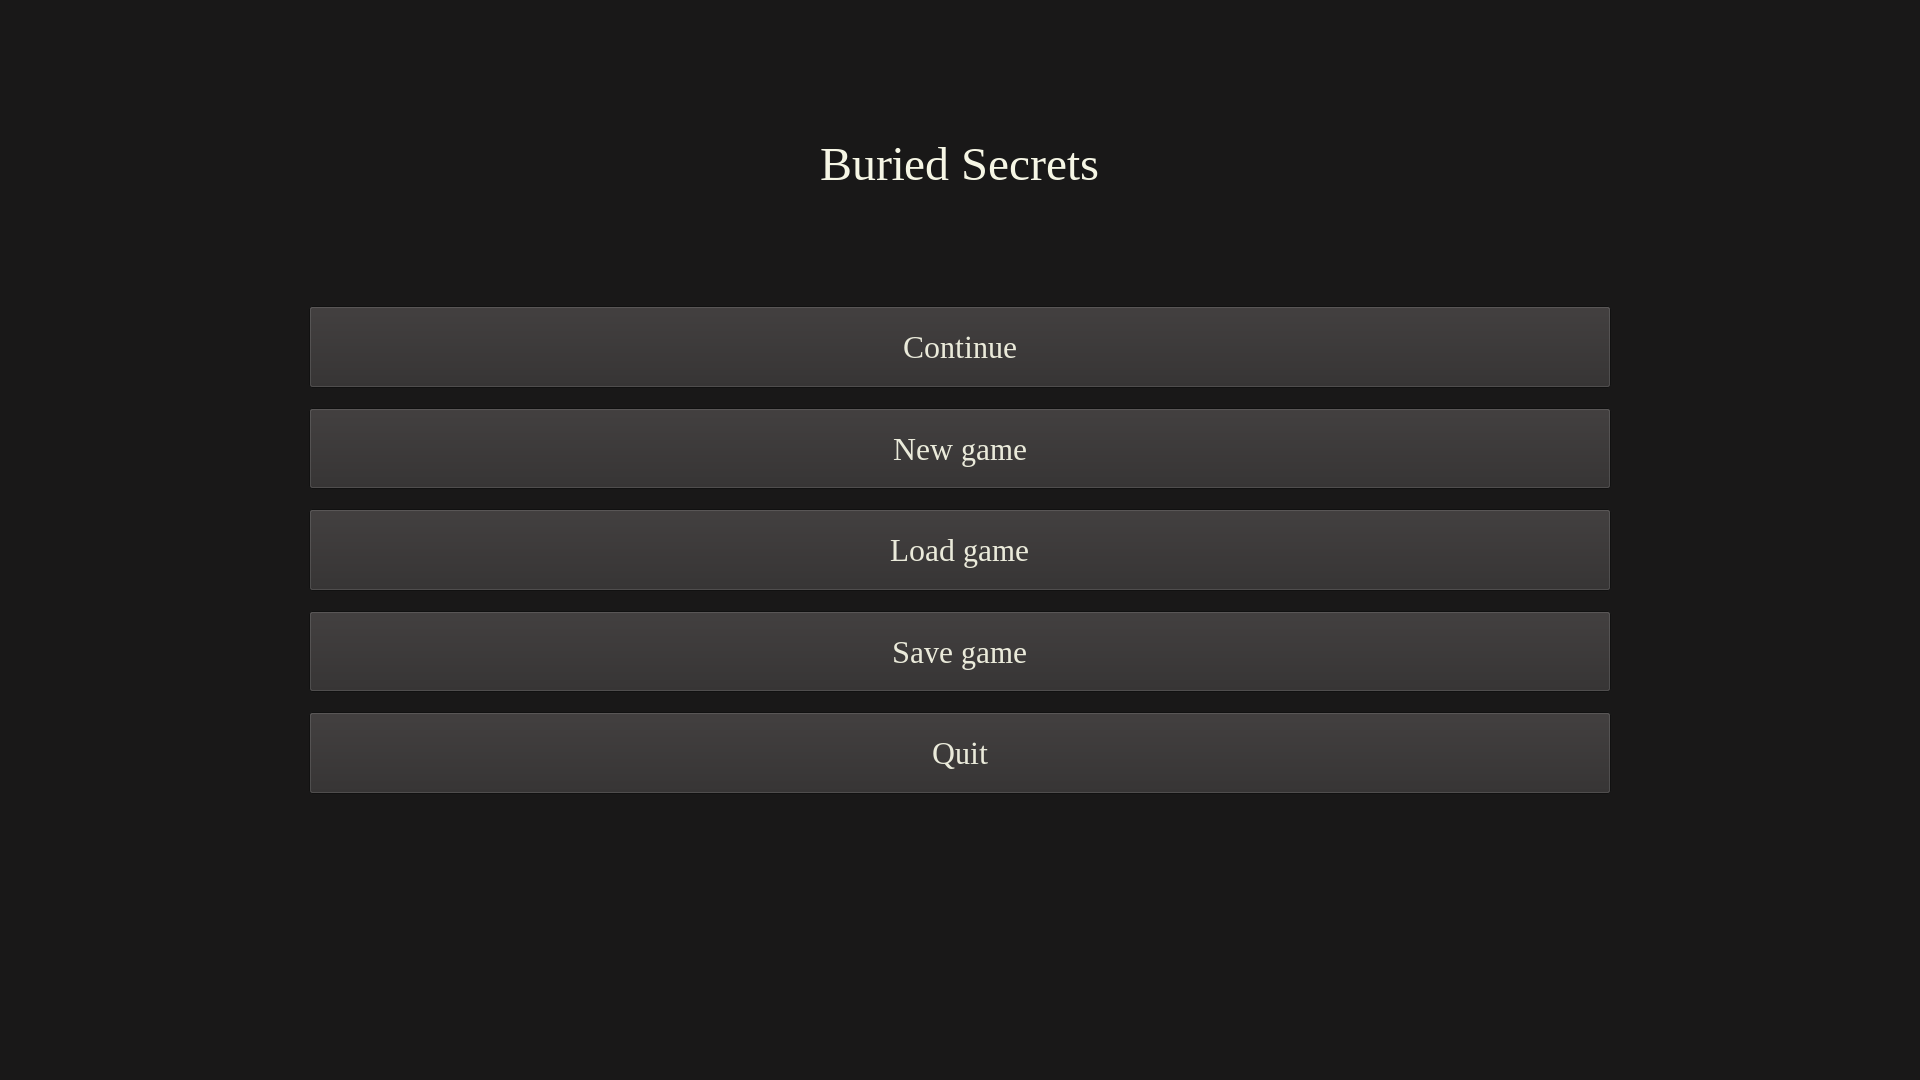
\includegraphics[scale=0.22]{MainMenu.png}
	\caption{Menu główne gry.}
      \end{figure}

    \subsection{Okno gry}
      Podczas gry użytkownik ma przed sobą planszę z~obiektami gry, którymi zarządza przy użyciu myszki, a przy brzegach ekranu znajdują się panele,
      dzięki którym gracz wydaje część poleceń oraz~poznaje stan gry. Głównym zadaniem planszy jest śledzenie stanu gry oraz~zaznaczanie i~wydawanie poleceń
      własnym jednostkom. Jednostki mogą być zaznaczane zarówno przez klikanie i~przeciąganie myszką na~mapie jak i~przez użycie skrótów klawiszowych.
      Poszczególne jednostki mogą zostać wybrane dzięki klawiszom funkcyjnym (F1 - F12), a klawiszom numerycznym można przyporządkować całe grupy jednostek.
      Polecenia wydawane jednostkom dzielą się na~dwie grupy:
      \begin{description}
       \item[Polecenia podstawowe] tj. atak, ruch, wejście/wyjście z~lokacji
       \item[Polecenia specjalne] tj. leczenie sojusznika, postawienie/złożenie fortyfikacji lub~obozu
      \end{description}
      Dokładne polecenie jakie zostanie wydane jednostkom zależy od tego, kogo gracz wcześniej zaznaczył, gdzie kliknął oraz~której grupy poleceń użył.
      \\\ \\ \noindent
      Poniżej zostały opisane panele, które znajdują się w~oknie gry.

      \subsubsection{Panel jednostek}
	Zawiera informacje o~obecnym stanie jednostek, pozwala przełączać się pomiędzy nimi i~otwierać okno szczegółowych informacji o~jednostce
	(więcej o~oknie poniżej). Okna pojawiające się podczas gry nie przesłaniają nigdy tego panelu, co~pozwala na~kontekstową zmianę jednostek
	w zakresie danego okna (np. zamiana postaci przy oglądaniu szczegółów o~jednostkach). Jest położony na~górze ekranu.

      \subsubsection{Panel frakcji}
	Wyświetla podstawowe informacje o~frakcji gracza i~umożliwia otwieranie okien dziennika, obozu oraz~wyjście do menu głównego.
	Znajduje się w~prawym dolnym rogu ekranu.
      \subsubsection{Panel zachowania}
	Pozwala na~zmianę zachowania obecnie zaznaczonych jednostek. Przylega do panelu frakcji.
      \subsubsection{Panel powiadomień}
	Miejsce na~ekranie, gdzie pojawiają się powiadomienia o~wszystkich istotnych dla użytkownika wydarzeniach gry. Jest położony w~lewym górnym rogu.

      \begin{figure}[htbp]
	\centering
	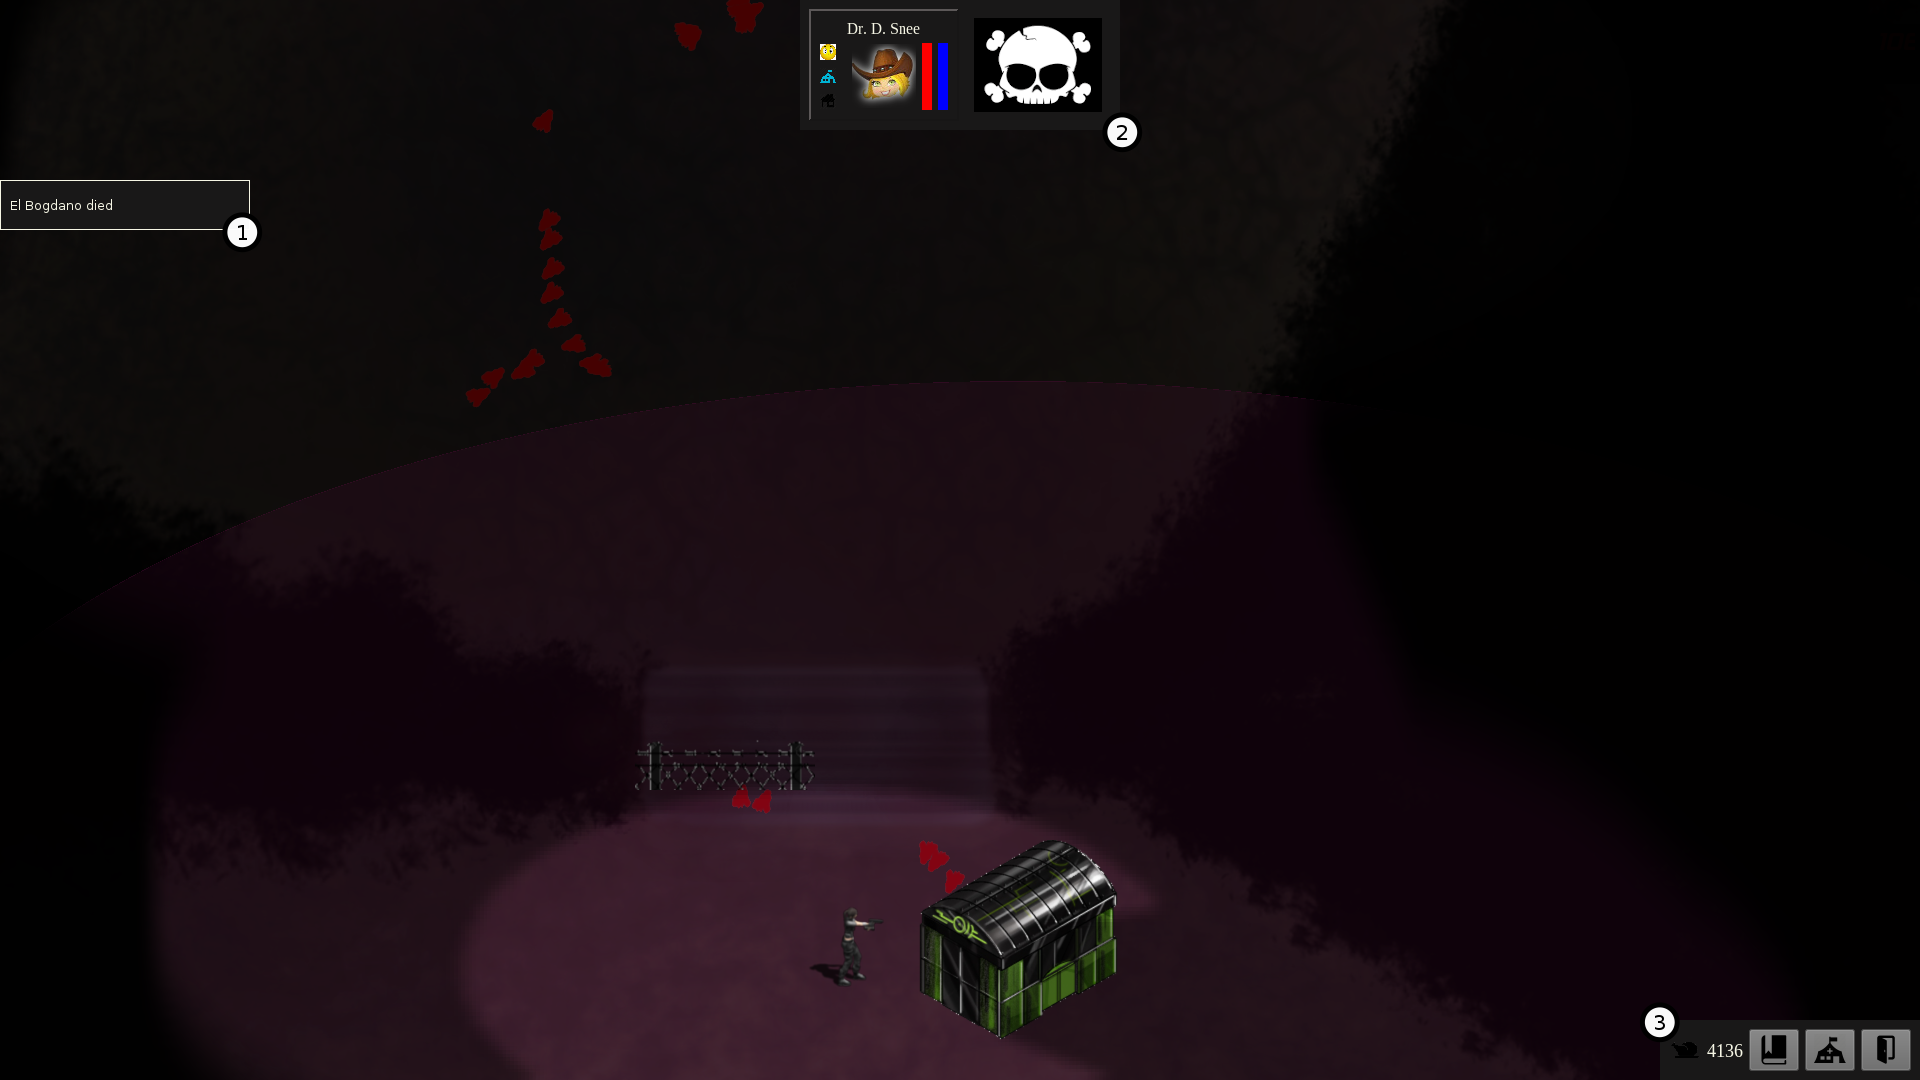
\includegraphics[scale=0.22]{Game.png}
	\caption{Okno gry (cyfry odpowiadają opisom poniżej).}
      \end{figure}

      \begin{enumerate}
       \item Panel powiadomień
       \item Panel jednostek
       \item Panel frakcji
      \end{enumerate}

    \subsection{Okna wewnątrz gry}

      \begin{figure}[htbp]
	\centering
	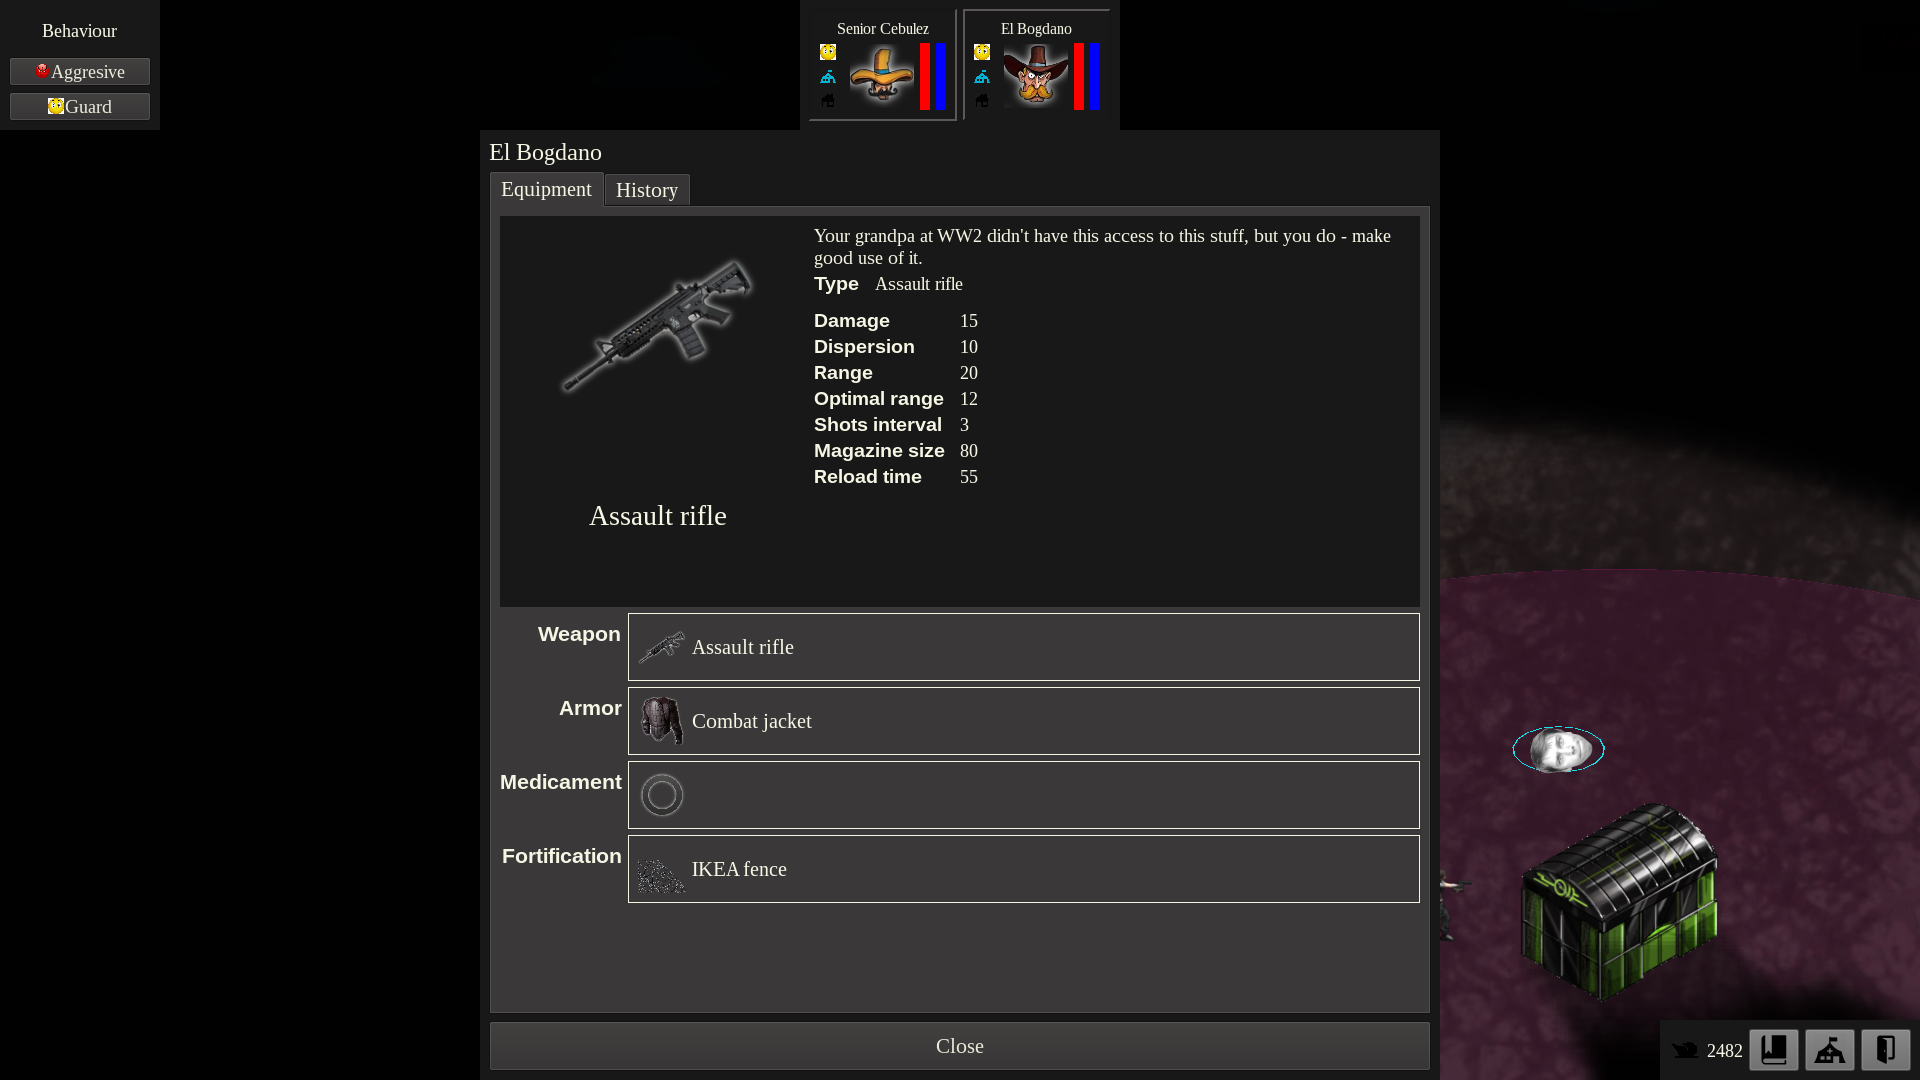
\includegraphics[scale=0.22]{Window.png}
	\caption{Przykładowe okno wewnątrz gry (Okno jednostki).}
      \end{figure}

      \subsubsection{Okno jednostki}
	Zawiera szczegółowe informacje o~wybranej jednostce gracza. Pozwala poznać jej wyposażenie, historię oraz~szczegółowe statystyki i~atrybuty.
      \subsubsection{Okno obozu}
	Pozwala na~obejrzenie ekwipunku obozu oraz~umożliwia konstruowanie nowych przedmiotów z~posiadanych części.
      \subsubsection{Okno dziennika}
	Dziennik zawiera wpisy o~wszystkich istotnych wydarzeniach zachodzących podczas gry. Służy do wygodnego przeglądania długich wpisów jak na~przykład
	opisów aktualnych zadań.
      \subsubsection{Okno wymiany z~obozem}
	Jest to specjalne okno, pojawiające się wtedy, gdy jednostka gracza odwiedzi własny obóz. Pozwala tej jednostce na~wymianie własnego ekwipunku z~bazą.
	Wymiana odbywa się metodą \emph{przeciągnij i~upuść} (\emph{drag-and-drop}).


  \section{Grafika}
    Wszystkie elementy gry rysowane na~mapie jak i~sama mapa są obsługiwane oddzielnie tzn. stanowią odrębną część programu, niezależną od interfejsu i~logiki gry.
    Poniżej opisano główne składowe grafiki.
    \subsection{Perspektywa}
      \begin{figure}[htbp]
	\centering
	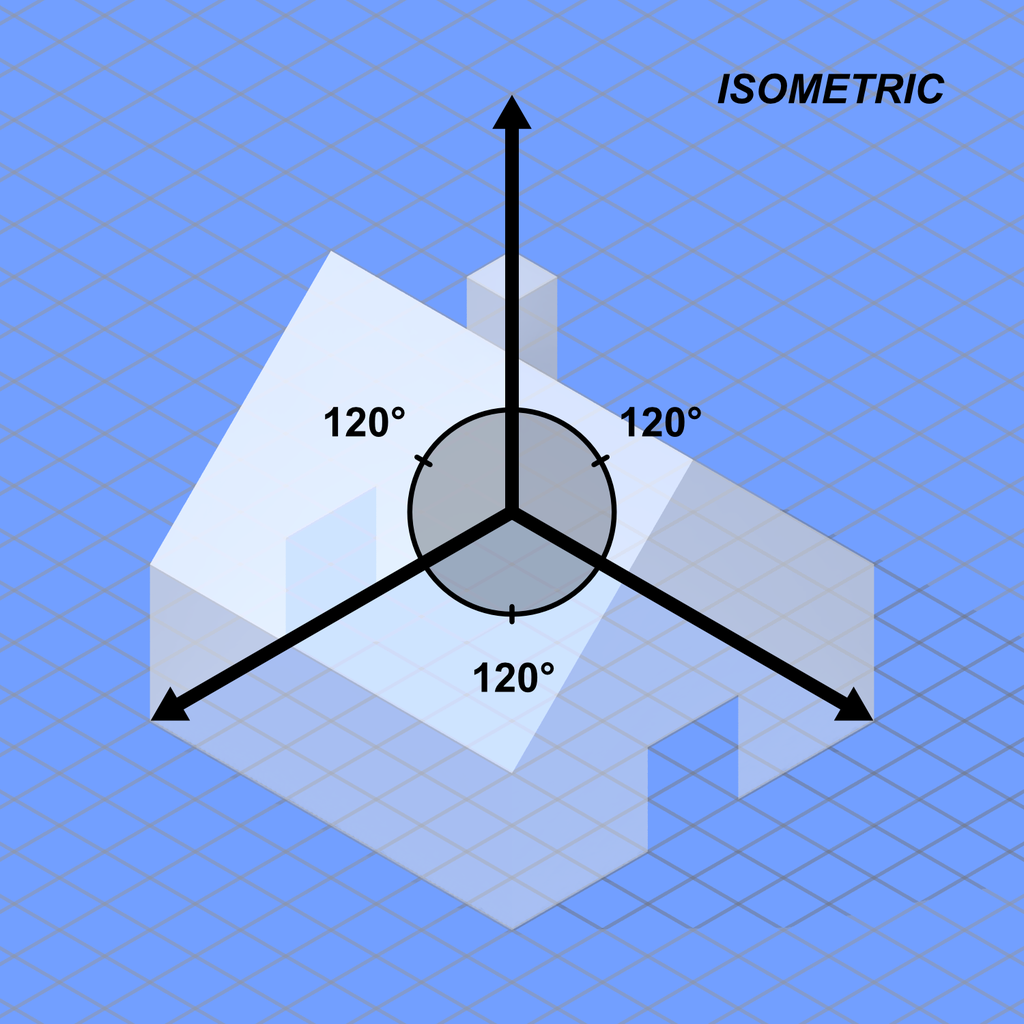
\includegraphics[scale=0.25]{izo.png}
	\caption{Perspektywa izometryczna\protect\footnotemark}
      \end{figure}

      \footnotetext{Grafika na~licencji CC-BY-SA wykonana przez \emph{SharkD} 
	\url{http://en.wikipedia.org/wiki/File:Graphical_projection_comparison.png#/media/File:Blue_house_isometric_projection.png}}
      Elementy gry rysowane są w~uproszczonym wariancie perspektywy izometrycznej.
      Przedstawienie świata w~ten sposób daje wrażenie dodatkowego, trzeciego wymiaru. Takie rozwiązanie wymusza przygotowanie tekstur
      postaci, budynków, elementów mapy i~samego podłoża w~przyjętej perspektywie, ale na~poziomie
      zawartości kończy się większość komplikacji. Kolejną z~konsekwencji przyjętego rzutu jest konieczność dodatkowego tłumaczenia
      współrzędnych między ekranowymi i~logicznymi.

      Dla lepszego imitowania trzech wymiarów, założyliśmy że każdy obiekt w~grze może być zwrócony w~jednym z~8 kierunków
      (co $45\degree$). Oznacza to, że dla obiektów poruszających się po planszy muszą być przygotowane osobne grafiki dla każdego kierunku.

    \subsection{Poziomy widoczności}
      Jako że kładliśmy nacisk na~taktyczny aspekt gry, podjęliśmy decyzję o~wykorzystaniu trzech poziomów widoczności. 
      \begin{enumerate}
       \item Obszary wokół kontrolowanych przez gracza jednostek są doskonale widoczne.
       \item Obszary obecnie poza zasięgiem widzenia, ale kiedyś już odwiedzone, są wyszarzone i~widać na~nich jedynie statyczne obiekty.
       \item Obszary nigdy nie odkryte są kompletnie niewidoczne.
      \end{enumerate}

      \begin{figure}[htbp]
	\centering
	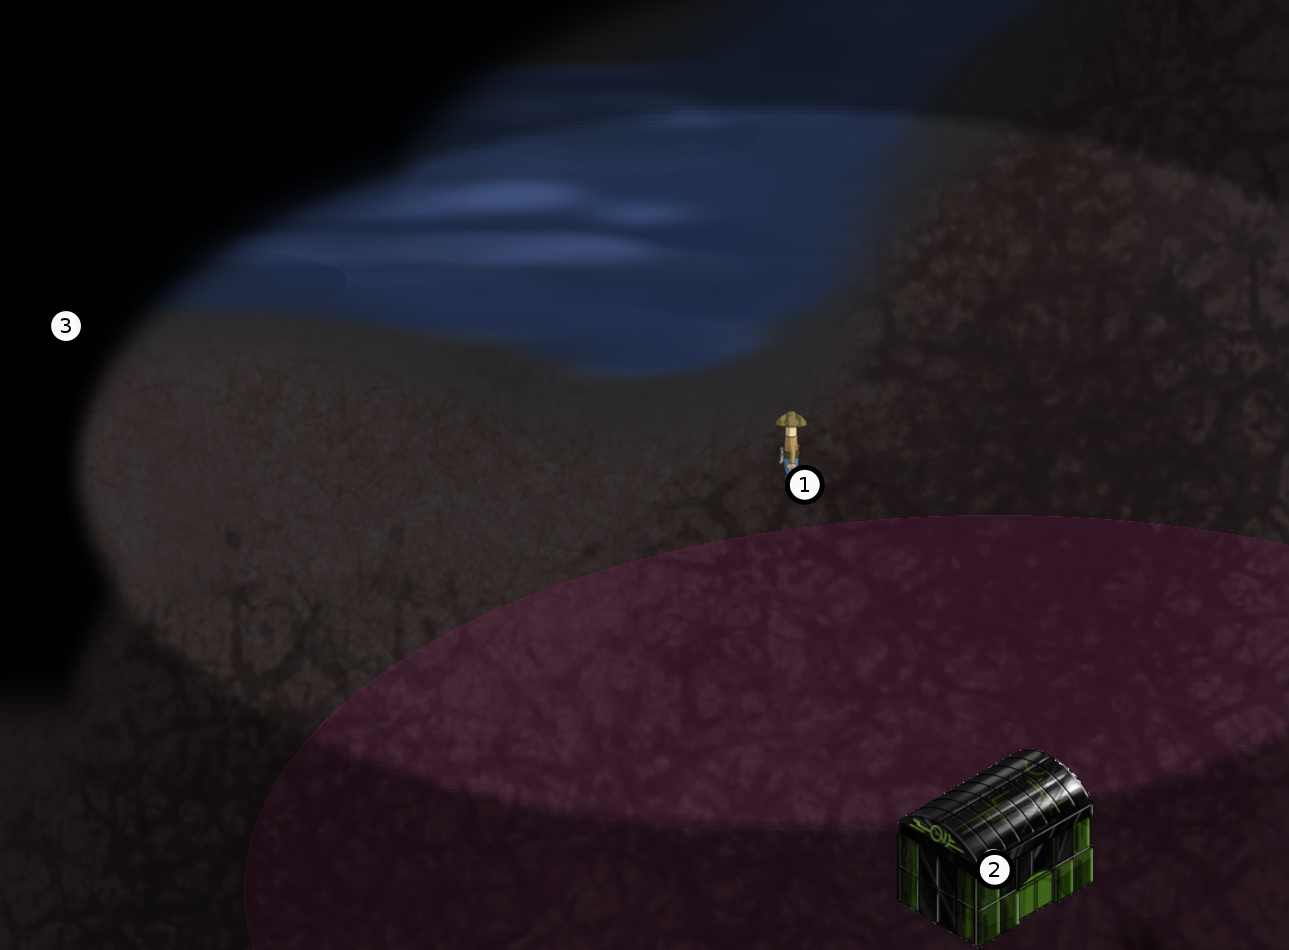
\includegraphics[scale=0.4]{fow.png}
	\caption{Poziomy widoczności w~grze (cyfry odpowiadają opisom powyżej).}
      \end{figure}

  \section{Analiza podobnych gier}
    Mechanika naszej gry była wymyślana od podstaw, z~możliwie małą ilością zapożyczeń z~innych tytułów. Możemy jednak wskazać
    kilka przykładów gier, które zawierają pewne elementy wspólne z~naszym projektem.
    \subsection{Gry oparte na~\emph{Commandos: Behind Enemy Lines}}
      \emph{Commandos: Behind Enemy Lines} jest pierwszą grą z~małego podgatunku taktycznych gier skradanych. Podobnie jak
      w~naszym projekcie, gracz steruje niewielką liczbą jednostek o~wyspecjalizowanych umiejętnościach i~stara się wykonywać skomplikowane
      misje na~planszy taktycznej, widzianej w~rzucie izometrycznym. Wszystkie postaci mają indywidualną historię i~są powiązane
      z~fabułą gry. Inny ważnym podobieństwem jest realizacja gry w~czasie rzeczywistym.

      Główna różnica polega na~tym, że \emph{Commandos: Behind Enemy Lines} stawia o~wiele większy nacisk na~ukrywanie się postaci, unikanie walki
      i~cierpliwe, długotrwałe planowanie każdego ruchu. Aby wzmocnić ten efekt, wykorzystano wykrywanie wrogich jednostek na~podstawie słuchu,
      graficzne zaznaczanie pola widzenia wroga, trójkątny kształt pola widzenia, różne tempa przemieszczania się jednostek.
      Naszym założeniem projektowym było unikanie powolnej rozgrywki i~realizacja gry z~dużą ilością bezpośredniej, dynamicznej walki.

    \subsection{\emph{Fallout Tactics}}
      Jest to kolejna gra, w~której gracz steruje kilkoma, wyspecjalizowanymi jednostkami. Podobnie jak w~\emph{Buried Secrets}, główny nacisk rozgrywki
      położony jest na~taktyczną walkę i~szybkie pozbywanie się wrogów. Można też wskazać podział rozgrywki na~pojedyncze zadania,
      realizowane na~mapie izometrycznej.

      Główne różnice to możliwość interakcji z~innymi postaciami na~ekranie (sprzedawcy), wielopoziomowe plansze, turowy tryb walki. Oprócz tego,
      w~grze \emph{Fallout Tactics} gracz ma większą swobodę w~wyborze postaci, którymi będzie grał i~nie są one aż tak ściśle powiązane z~fabułą.

\chapter{Narzędzia i~metodologia pracy}
  \section{Użyte biblioteki}
    \subsection{Qt}
      Do rysowania graficznego interfejsu użytkownika wykorzystujemy platformę Qt\cite{QT} w~wersji 5. Dokonaliśmy takiego wyboru
      ze względu na~wcześniejsze doświadczenie z~nim w~innych projektach wykonywanych w~ramach Indywidualnego Projektu Programistycznego
      i~Inżynierii Oprogramowania. Istotną zaletą Qt jest również wieloplatformowość.

      Ponieważ kontenery w~Qt znacząco rozszerzają swoje odpowiedniki z~biblioteki standardowej C++ zdecydowaliśmy się na~ich użycie
      w~całym projekcie. Przydatnymi elementami Qt wykorzystywanymi w~naszej grze były również: system zarządzania zasobami,
      system zarządzania plikami na~dysku oraz~mechanizm sygnałów i~slotów. Ten ostatni z~uwagi na~narzut na~wydajność został 
      wykorzystany jedynie przy implementacji interfejsu użytkownika.

    \subsection{SFML}
      Do wyświetlania grafiki w~naszym projekcie używamy biblioteki SFML\cite{SFML} (Simple and Fast Multimedia Library) w~wersji
      2.2. Rysowanie grafiki z~użyciem GPU w~Qt nie spełniało wszystkich naszych potrzeb pod kątem wydajności i~oferowanych funkcjonalności.
      Po krótkich poszukiwaniach wybór padł na~SFML. Zaletami były: prostota, silna obiektowa architektura, nastawienie na~użycie w~grach,
      wieloplatformowość (wersja 2.2 wspiera nawet platformy mobilne) i~możliwość ewentualnego zejścia na~niższy poziom abstrakcji.
      Z perspektywy czasu możemy stwierdzić, że SFML spełnił wszystkie nasze oczekiwania w~zakresie oferowanych możliwości.

    \subsection{Box2D}
      Pomimo taktycznego charakteru gry, bez dużej liczby symulacji zjawisk fizycznych, zdecydowaliśmy się na~wykorzystanie
      w~projekcie zewnętrznego silnika fizycznego. Miał on udostępniać płynne przemieszczanie się obiektów, wygodne
      zapytania o~obiekty znajdujące się w~danym obszarze, detekcję kolizji, oraz~sprawdzanie obiektów znajdujących się na~linii
      strzału. Stwierdziliśmy, że spośród dostępnych silników najlepiej do naszych potrzeb pasuje Box2D\cite{BOX}, niewielki,
      otwarty silnik fizyki dwuwymiarowej. Większość konkurencyjnych produktów była albo zbyt skomplikowana albo oferowała tylko
      symulacje 3D. Wstępne testy wydajności tej biblioteki przeprowadziliśmy na~projekcie \texttt{Dziekan}, prostej grze powstałej
      w~ramach Inżynierii Oprogramowania.

  \section{Metodologia pracy}
    Pracę nad naszym projektem rozpoczęliśmy od sporządzenia wizji gry, a w~szczególności jej mechaniki. Te jak i~kolejne
    ustalenia m.in. dotyczące grafiki czy architektury formułowaliśmy i~dokumentowaliśmy przy użyciu \emph{Google Docs}\footnote{Aplikacja 
    sieciowa od firmy \emph{Google} do współdzielenia i~edycji dokumentów tekstowych (docs.google.com)}. Dawało to nam kontrolę i~przejrzystość
    założeń projektowych przez cały czas pracy nad grą. Ponadto organizowaliśmy cotygodniowe spotkania całego zespołu, gdzie omawialiśmy stan projektu
    i~planowaliśmy kolejne działania rozdzielając zadania do wykonania przed kolejnym spotkaniem. Do kontrolowania postępu wspomnianych zadań korzystaliśmy
    z~serwisu \emph{Asana}\footnote{Aplikacja sieciowa do zarządzania zadaniami przy projektach wieloosobowych. (asana.com)}.

    Do pracy nad kodem programu używaliśmy systemu kontroli wersji \emph{Git} w~połączeniu z~serwisem \emph{Github}\footnote{Hostingowy
    serwis internetowy przeznaczony dla projektów programistycznych wykorzystujących system kontroli wersji Git. (github.com)}, którego używaliśmy
    do robienia code review. Przed rozpoczęciem pracy nad kodem źródłowym ustaliliśmy obowiązujące formatowanie kodu i~umieściliśmy je w~repozytorium.

    Aby testować na~bieżąco efekty naszej pracy zdecydowaliśmy się na~prowadzenie regularnych playtestów gry. Pozwalało nam to określić,
    czy rozwijamy nasz projekt w~dobrym kierunku oraz~dostarczało pomysłów na~nowe funkcjonalności i~rozwiązania pojawiających się problemów.
    Więcej informacji o~playtestach znajduje się w~rozdziale poniżej.

\chapter{Architektura}
  \section{Ogólny opis}
    Program składa się z~następujących modułów:
    \begin{itemize}
      \item \texttt{Common}
      \item \texttt{DataManager}
      \item \texttt{DebugManager}
      \item \texttt{GameObjects}
      \item \texttt{General}
      \item \texttt{Graphics}
      \item \texttt{Mind}
      \item \texttt{PhysicsEngine}
      \item \texttt{UserInterface}
    \end{itemize}

    Głównym modułem jest \texttt{General} -- to on inicjuje działanie wszystkich pozostałych modułów, reaguje na
    polecenia odczytu i~zapisu gry oraz~przekazuje część informacji pomiędzy nimi.

    Moduł \texttt{DataManager} zajmuje się wczytywaniem i~przechowywaniem danych. Dane stanowią głównie informacje
    o~obiektach przetrzymywane w~\texttt{GameObjects}. Uniwersalne informacje dzielone pomiędzy różnymi instancjami danego
    typu obiektów są przetrzymywane w~prototypach skąd instancje mogę je pobierać. Zarządzaniem obiektami tj. zmianą ich wartości,
    dynamicznym ich dodawaniem i~usuwaniem zajmuje się moduł \texttt{Mind}. \texttt{Mind} zawiera logikę całej gry wraz z~pętlą gry
    realizowane przez tzw. animatory - klasy odpowiedzialne za pewne, dokładnie ustalone działanie na~obiektach gry.
    Animatory wywoływane są okresowo i~operują wyłącznie na~przydzielonych im obiektach.

    Obrazowaniem stanu gry i~interfejsu na~ekranie zajmują się moduły \texttt{Graphics} i~\texttt{UserInterface}.
    \texttt{Graphics} ma dostęp do modułu \texttt{Mind}, dzięki czemu możliwe jest szybkie sprawdzanie stanu
    gry i~wykonanie odpowiednich zmiany. \texttt{UserInterface} reaguje na~polecenia gracza, korzystając przy tym z~interfejsów modułów
    \texttt{General} i~\texttt{Mind}.

    Do silnika gry należy również pomocniczy moduł \texttt{PhysicsEngine} wspierający zarządzanie obiektami w~dwuwymiarowej przestrzeni.
    \texttt{PhysicsEngine} jest głównie wykorzystywany przez \texttt{Mind}. Pomocnicze funkcje, zmienne wyliczeniowe i~ich słowne 
    odpowiedniki znajdują się są w~module \texttt{Common}, zaś \texttt{DebugManager} udostępnia funkcje służące do wypisywania wiadomości
    o~różnym priorytecie i~charakterze w~czytelnej postaci.

    \begin{figure}[htbp]
      \centering
      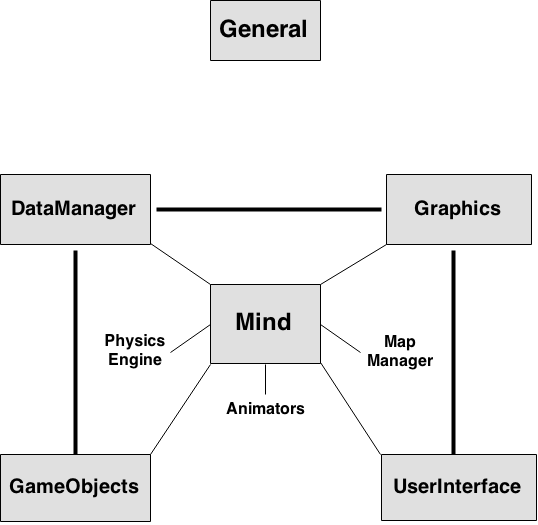
\includegraphics[scale=0.5]{diagram-klas.png}
      \caption{Uproszczony diagram zależności pomiędzy modułami.}
    \end{figure}

  \section{Moduł \texttt{General}}
    Moduł \texttt{General} łączy wszystkie pozostałe moduły i~udostępnia podstawowe funkcje dotyczące wczytywania i~zapisywania
    mapy. Podczas jego inicjalizacji tworzone są również moduły \texttt{DataManager}, \texttt{UserInterface} i
    \texttt{DebugManager}.

    W~momencie rozpoczęcia rozgrywki na~ustalonym poziomie, tworzone są moduły \texttt{PhysicsEngine},
    \texttt{Mind}, \texttt{Graphics} oraz~interfejs dla danego poziomu w~\texttt{UserInterface}. Elementy te są niszczone i~tworzone
    ponownie przy każdej zmianie poziomu. Upraszcza to zdecydowanie zarządzanie pamięcią nie powodując odczuwalnego spadku wydajności.

  \section{Moduł \texttt{GameObjects}}
    Stan gry przetrzymywany jest w~module \texttt{GameObjects}. Znajdują się tutaj zarówno wszystkie obiekty widoczne na
    mapie, jak i~wszelkiego rodzaju wpisy w~dzienniku, zadania, itd. Każdy obiekt jest serializowalny i~posiada swój unikalny
    identyfikator oraz~ma przypisany prototyp z~modułu \texttt{DataManager}. Obiekty posiadają również możliwość przechowywania
    tymczasowe wartości, niezbędnych do działania gry.

    Konkretne rodzaje obiektów występujących w~grze wraz z~informacjami, które przetrzymują:
    \begin{itemize}
      \item \texttt{Faction} -- ilość zapasów żywności, zasięg obozu, lista jednostek przynależnych do danej
	frakcji, dziennik i~ekwipunek obozu tej frakcji,
      \item \texttt{Equipment} -- lista przedmiotów znajdujących się w~ekwipunku, a także funkcje, jakie w~nim pełnią,
      \item \texttt{Item} --  ile razy i~jak często można danego przedmiotu używać,
      \item \texttt{Unit} -- różne statystyki jednostek, obecna ścieżka, po której jednostka się porusza, ustawione nastawienie,
      \item \texttt{Journal} -- lista wpisów do dziennika,
      \item \texttt{JournalEntry} -- data, tekst, tytuł i~rodzaj wpisu do dziennika,
      \item \texttt{Quest} -- tytuł, warunki początkowe, sukcesu i~porażki danego zadania,
      \item \texttt{Location} -- lista przedmiotów i~jednostek znajdujących się w~danej lokacji, maksymalna pojemność lokacji.
    \end{itemize}

    %Jeśli mówimy że MM jest modułem to niech będzie tak nazwany i będzie stylizowany na równi z innymi%
  \section{Moduł \texttt{Mind}}

    \texttt{Mind} odpowiada za zarządzanie obiektami gry i posiada wszelkie informacje o jej stanie. 
    Każdy obiekt gry jest tworzony w tym module, rejestrowany i przechowywany. Gdy dowolny inny moduł potrzebuje dostępu do 
    obiektu gry, uzyskuje go od \texttt{Mind}, poprzez podanie identyfikatora. Pozwala to uporządkować zarządzanie pamięcią
    i uprościć model zmieniania stanu gry. 

    Obiekt typu \texttt{Mind} tworzony jest od nowa na początku każdej misji, aby uniknąć przekazywania nieusuniętych danych
    między rozgrywkami. Podczas jego tworzenia, powstają dodatkowo moduły \texttt{Animators} oraz \texttt{MapManager}, które 
    są ściśle powiązane z aktualną grą. 	
	
  \section{Moduł \texttt{Animators}}
    \texttt{Animatory} są naszym autorskim rozwiązaniem problemów występujących przy tworzeniu pętli gry. Każdy \texttt{Animator}
    odpowiada za realizację niewielkiego, atomowego fragmentu zachowania pewnego zbioru obiektów gry. Przykładami takich
    fragmentów są zmiana klatki animacji, przesunięcie obiektu na planszy, śmierć postaci.
    
    Gdy powstaje obiekt, zostaje on dodany do list obiektów odpowiednich \texttt{Animatorów}. Następnie, co pewien stały czas, 
    \texttt{Animatory} aktualizują jego stan. Pozwala to elastycznie wybierać podzbiór zachowań, aplikowanych do poszczególnych
    obiektów tego samego typu. 
    
    Moduł \texttt{Animators} odpowiada za stworzenie wszystkich wykorzystywanych \texttt{Animatorów}, udostępnienie interfejsu
    dodawania i usuwania z nich obiektów gry oraz okresowe ich aktualizowanie. 
  \section{Moduł \texttt{MapManager}}
    \texttt{MapManager} jest modułem zajmującym się wszystkim co~związane z~przetwarzaniem, utrzymywaniem oraz~udostępnianiem
    informacji o~mapie. Dwie główne funkcjonalności to utrzymywanie informacji o~zasięgu widoczności jednostek wszystkich
    frakcji oraz~wyszukiwanie ścieżek.

    Informacje o~jakichkolwiek zmianach widoczności są do \texttt{MapManager} przekazywane przez jeden z~animatorów, a z~tego miejsca
    przekazywane dalej do modułu \texttt{Graphics}. Z tego powodu \texttt{MapManager} udostępnia metody pozwalające na~pobranie
    zbioru wszystkich zmian widoczności z~pewnego przedziału czasowego. Dzięki takiej budowie, mimo że animatory oraz~pętla 
    renderująca grafiki działają z~inną częstotliwością, informacja o~zmianie widoczności nigdy nie ginie.

    Do wyliczania ścieżek używaliśmy pierwotnie algorytmu A*\cite{A*} z~kilkoma modyfikacjami pozwalającymi na~użycie go do mapy
    niepodzielonej na kafelki (logiczne fragmenty równych rozmiarów dzielące mapę). W~trakcie playtestów okazało się jednak,
    że~to~rozwiązanie nie jest wystarczająco wydajne. Jako usprawnienie zaimplementowaliśmy wtedy algorytm HPA*\cite{HPA} oraz~
    wprowadziliśmy heurystyki zmniejszające częstotliwość zapytań o~ścieżki.

  \section{Moduł \texttt{DataManager}}
    W~module \texttt{DataManager} znajduje się cała logika wczytywania i~zapisywania danych. Dla wygody, dla plików z
    danymi o~grze, przyjęliśmy popularny format \emph{JSON}. Pozostałe dane (pliki graficzne) przechowywane są w~formacie
    binarnym. Takie rozwiązanie ułatwia parsowanie przetrzymywanych danych, kosztem braku szczegółowej ich walidacji.

    Moduł \texttt{DataManager} jest inicjalizowany przez \texttt{General} na~początku programu. Wczytywane są wtedy wszystkie dane
    niedotyczące konkretnej mapy, tzn. prototypy i~informacje o~dostępnych plikach graficznych. W~prototypach znajdują się 
    bazowe informacje o~obiektach gry. \texttt{DataManager} oferuje do nich dostęp za pomocą odpowiedniego interfejsu.

  \section{Moduł \texttt{PhysicsEngine}}
    \texttt{PhysicsEngine} jest jednym z~najmniejszych modułów naszego projektu. Udostępnia ogólny, niezależny od
    wewnętrznej implementacji interfejs funkcjonalności silnika fizycznego oraz~jedną jego implementację, wykorzystującą bibliotekę Box2D.
    Pozwala na~proste operowanie na~obiektach gry (dodawanie ich do silnika, przesuwanie, obracanie), symulowanie ruchu obiektów,
    obsługę ich zderzeń, realizację zapytań o~obiekty na~planszy (zapytania AABB), śledzenie torów poruszających się pocisków (ray tracing).
    Aktualizacja stanu silnika fizycznego odbywa się przy użyciu jednego z~animatorów.

    Wszystkie obiekty znajdujące się na~planszy mają swoją osobną reprezentację w~\texttt{PhysicsEngine}, który jest jedynym miejscem
    przechowującym informacje o~fizycznych właściwościach obiektów, takich jak położenie czy prędkość. Geometria dodawanych obiektów
    jest ustalana na~podstawie ich prototypów i~jest stała przez cały czas trwania gry.

  \section{Moduł \texttt{Graphics}}
    Moduł \texttt{Graphics} zawiera logikę rysowania mapy wraz ze wszystkimi jej obiektami. Operuje na
    abstrakcyjnych graficznych reprezentacjach następujących elementów:
    \begin{itemize}
     \item logicznych obiektów gry (jednostek, budynków itd.)
     \item efektów (zaznaczenie jednostki, zasięg działania bazy itd.)
     \item decali\protect\footnotemark (ślad po strzale, ślad krwi itd.)
    \end{itemize}
    \footnotetext{Decale -- efekty wizualne rysowane na~powierzchni oteksturowanego już obiektu.}

    Głównym założeniem modułu \texttt{Graphics} było, aby logika była od niego kompletnie niezależna, a tym samym możliwe
    było szybkie jej podmienienie. Daje to możliwość ewentualnej kompletnej zmiany szaty wizualnej gry (np. reazlizowanej w~3D)
    relatywnie małym kosztem. Dodatkowym powodem było zarządzanie ryzykiem jakim było korzystanie z~SFML, którego wcześniej
    nie używaliśmy.

    Rysowanie odbywa się w~pętli niezależnej od logiki gry -- istnieje osobny zegar, który generuje
    przerwania z~najmniejszym możliwym interwałem na~jaki pozwala sprzęt przy aktualnym obciążeniu. Cała gra w~obecnym
    stadium rozwoju działa w~jednym wątku, zatem w~praktyce i~ten timer jest ograniczony resztą programu. Takie
    rozwiązanie pozwala nam jednak na~łatwiejsze zarządzanie chronologią zdarzeń oraz~daje możliwość potencjalnego
    przeniesienia rysowania do~oddzielnego wątku bez dużych zmian w~architekturze.

    \subsection{Rysowanie}
      Logika rysowania przedstawia się następująco:
      \begin{enumerate}
       \item Pobierz listę aktualnie widocznych obiektów z~logiki (używając modułu fizycznego).
       \item Usuń z~niej obiekty niewidoczne (przesłonięte mgłą wojny itd.).
       \item Dodaj potrzebne efekty w~poprawnej kolejności
      \end{enumerate}

    \subsection{Zarządzanie pamięcią}
      Tekstury są ładowane do pamięci karty graficznnej dopiero jeśli są potrzebne do wyświetlenia jakiegoś
      obiektu. Początkowo mieliśmy wątpliwości co~do wydajności tego rozwiązania, ale praktyczne testy pokazały, że
      takie doładowywanie danych z~pamięci operacyjnej do pamięci karty jest niezauważalne.

    \subsection{Entities}
      Każdy obiekt, który ma być wyświetlony na~ekranie jest w~module \texttt{Graphics} tłumaczony na~\texttt{GraphicalEntity}, które
      zapewnia poziom abstrakcji właściwy grafice, ukrywając szczegóły logiki. Dopiero na~takich abstrakcyjnych obiektach operuje grafika.

    \subsection{Effects}
      W~grze wyświetlamy różne efekty, które nie dają się reprezentować logicznymi obiektami, zatem nie mogą być bezpośrednio tłumaczone
      na~\texttt{Entity}. Efekty dzielą się na~dwie rozłączne grupy: towarzyszące jakimś obiektom (np. efekt zaznaczenia jednostki) oraz~
      od nich niezależne (np. efekt kursora po wydaniu komendy ruchu). Pierwszy rodzaj efektów jest związany z~konkretnymi obiektami i~jest
      rysowany względem ich współrzędnych. Drugi jest traktowany jak \texttt{Entity}, dzięki czemu trafia do tej samej puli obiektów rysowanych
      na~ekranie, jednak jest rysowany niezależnie.

    \subsection{Decals}
      W~naszym projekcie wprowadziliśmy system decali, służący do rysowania tylko po teksturze mapy. Na chwilę obecną wykorzystujemy go do
      rysowania śladów krwi po trafionych strzałach, ale z~powodzeniem można go wykorzystać do tworzenia bardziej zaawansowanych efektów.

    \subsection{Poziomy widoczności}
      Poziomy widoczności jednostek (popularnie określane jako Fog of War) są trzymane na~dosyć małych teksturach ze względu na~ograniczenia
      niektórych kart graficznych. Aby wyświetlić wizualnie atrakcyjny efekt końcowy, po przeskalowaniu tekstur na~rozmiar ekranu
      (oraz uprzednim wykadrowaniu interesującego nas fragmentu) aplikowane są do nich shadery realizujące Gaussowskie rozmycie\cite{GB}
      uzyskując w~ten sposób atrakcyjny rezultat przy okazji zmniejszając istotnie ilość danych przesyłanych do karty graficznej.

  \section{Moduł \texttt{UserInterface}}
    Moduł \texttt{UserInterface} odpowiada za wyświetlanie graficznego interfejsu gry, przechwytywanie akcji użytkownika
    oraz~tłumaczenie tych akcji na~wywołania odpowiednich metod części logicznej. Ponadto przechowuje stan związany
    z~interfejsem, jak na~przykład aktualnie widoczny obszar mapy czy zbiór zaznaczonych jednostek.

    \texttt{User Interface} silnie korzysta z~biblioteki Qt, w~szczególności mechanizmu sygnałów i~slotów oraz~struktur danych
    tej biblioteki, co~znacząco ułatwia implementowanie interfejsu użytkownika. W~konsekwencji kod tego modułu zawiera wiele
    konwencji i~wzorców programistycznych używanych w~Qt.

    Głównymi modułami, z~którymi współdziała \texttt{UserInterface} są:
    \begin{itemize}
     \item \texttt{DataManager} -- wykorzystywany do pozyskiwania zasobów do wyświetlenia w~interfejsie użytkownika
     \item \texttt{Mind} -- wykorzystywany do uzyskiwania informacji o~globalnym stanie gry oraz~udostępnia poszczególne elementy \texttt{GameObjects}
     \item \texttt{GameObjects} -- wykorzystywane do przekazania części logicznej akcji gracza na~konkretnych obiektach gry
    \end{itemize}

    Poniżej zostały wymienione główne logiczne elementy tego modułu odpowiadające realizowanym przez niego zadaniom,
    co~przekłada się również na~podział w~kodzie programu:

    \begin{itemize}
     \item Rysowanie i obsługa: menu głównego, okna gry, okien wewnątrz gry,
     \item Obsługa zaznaczania obiektów gry,
     \item Ustalanie i~wydawanie komend jednostkom gracza,
     \item Wyznaczanie i~manipulacja widocznym obszarem mapy.
    \end{itemize}

  \section{Pozostałe moduły}
    W~naszym projekcie, poza wymienionymi powyżej, posiadamy jeszcze dwa moduły warte uwagi.
    \paragraph{Moduł \texttt{Common}}
      Zawiera metody wykorzystywane przez kilka modułów jednocześnie (np. związane z~geometrią), definicje stałych i~typów wyliczeniowych
      wraz z~metodami ich serializacji/deserializacji oraz~inne pomniejsze funkcjonalności.
    \paragraph{Moduł \texttt{DebugManager}}
      Zawiera zbiór metod do wypisywania na~konsolę informacji diagnostycznych.

  \chapter{Kamienie milowe}
    \section{Podstawowy silnik gry}
    Podstawowy silnik ukończyliśmy w~lutym i~zawierał dopracowany szkielet całej gry, system obiektów gry,
    logikę zarządzająca tymi obiektami, grafikę wyświetlania mapy gry oraz~szkielet interfejsu użytkownika.
    Na tym etapie ustaliła się jasna architektura programu, co~pozwalało nam ocenić, możliwości jakie
    daje taki projekt i~implementacja silnika. Przykładowo, wykorzystanie animatorów pozwalało nam w~wygodny
    i~elegancki sposób rozwiązać problemy związane z~obsługą zdarzeń czasu rzeczywistego, natomiast wymagało kontroli
    nad kolejnością wykonywania poszczególnych animatorów przez istniejące pomiędzy nimi zależności. Inny wniosek
    na~tym etapie dotyczył implementacji obiektów gry. Bardzo generalna struktura obiektów tj. przetrzymywanie
    ich~własności w~dynamicznej strukturze pozwalało na~szybkie zmiany, co~było częste w~tej~fazie projektu,
    ale~sprawiało trudności w~walidacji poprawności danych.
    Po~zaimplementowaniu podstawowego silnika byliśmy już zaznajomieni z~możliwościami zewnętrznych bibliotek,
    z~których korzystaliśmy, co~pozwoliło nam lepiej przewidzieć czas potrzebny na~zrealizowanie zaplanowanych
    funkcjonalności jak~i~ocenić wydajność naszego rozwiązania.

    \section{Pierwsza wersja gry}
    Pierwsza wersja gry była gotowa na~początku marca i~powstała w~związku z~przeprowadzonymi playtestami. Jej~głównym
    celem było umożliwienie graczowi możliwie bogatej interakcji z~grą. Wymagało to dodania podstawowych
    danych testowych tj. planszy, przedmiotów, jednostek, budynków, konstrukcji jak i~zależności pomiędzy nimi.
    W~efekcie gracz miał do dyspozycji testowy poziom polegający na~przejściu przez przygotowaną mapę wymagający
    przy tym zapoznania się z~podstawowymi mechanizmami rozgrywki.

    \section{Druga wersja gry}
    Kolejną wersję ukończyliśmy na~początku maja. Nanosiła poprawki błędów wykrytych podczas pierwszych testów, wprowadzała kilka nowych
    funkcjonalności oraz~modyfikowała istniejące. Dodaliśmy system zadań realizowanych przez gracza oraz~zmodyfikowaliśmy zasady modyfikowania
    ekwipunku. Na podstawie problemów z~przenoszeniem obozu zmieniliśmy mechanikę tej operacji, a dokładniej jednostka przestawiająca
    obóz od tej pory na~czas transportu obozu zamieniała się w~transporter (co zastąpiło dotychczasowe przenoszenie konstrukcji w~ekwipunku).
    Dołożyliśmy również nowy poziom stawiający gracza przed koniecznością bardziej defensywnej rozgrywki,
    co~pozwoliło zwiększyć znaczenie konstrukcji stawianych na~mapie przez gracza. Innym elementem, istotnie poprawiającym
    rozgrywkę było wprowadzenie wyszukiwania ścieżek, co~skutkowało bardziej intuicyjnym i~łatwiejszym w~sterowaniu
    zachowaniem jednostek. Wymienione zmiany pociągnęły ze sobą również zmiany w~interfejsie.

\chapter{Playtesty}
  \section{Założenia}
    Aby przetestować działanie i~odbiór naszą gry przez użytkowników przeprowadziliśmy playtesty. Główne ich cele to:
    \begin{itemize}
    \item Wyszukanie błędów działania
    \item Przetestowanie zaprojektowanej mechaniki
    \item Przetestowanie interfejsu użytkownika
    \item Zbadanie reakcji gracza
    \item Zbadanie strategii gracza
    \item Zbalansowanie gry
    \end{itemize}
    W~zależności od stadium rozwoju projektu kładliśmy nacisk na~różne z~wymienionych celów. Przykładowo interfejs użytkownika,
    ze względu na~zachodzące zmiany ulegał ciągłej zmianie stąd pracowaliśmy nad nim iteracyjnie przez cały czas, natomiast
    zbadanie strategii gracza było możliwe dopiero w~późniejszych testach. Istotnym elementem obu faz testów było uzyskanie
    informacji zwrotnej od~nowych testerów, nieznających koncepcji gry.

  \section{Faza I}
    Ta faza testów została przeprowadzona na~pierwszej wersji gry (opisana w~rozdziale \emph{Kamienie milowe})
    z~niepełnym zestawem funkcjonalności i~prototypowymi fragmentami grafiki. Skupiliśmy się na~przetestowaniu mechaniki
    i~interfejsu gry oraz~spisaniu istniejących błędów, ponieważ brak wszystkich funkcjonalności ograniczał nasze możliwości.
    Jednocześnie był to ostatni moment na~poważne zmiany logiki lub~dodanie nowych funkcji silnika.

    \subsection{Forma}
      Każdy test składał  się z~dwóch części: samodzielnej 15-20 minut gry
      oraz~swobodnej rozgrywce z~dozwoloną ingerencją koordynatora.

      Pierwsza część testu polegała na~indywidualnej grze na~ówcześnie gotowej planszy.
      Każdy gracz otrzymał wydrukowaną instrukcję gry (zawierającej sterowanie i~wstęp fabularny)
      i~powinien był sam zrozumieć cel oraz~zasady gry. W~tym czasie zespół udzielał podpowiedzi
      wyłącznie w~przypadku wyraźnych problemów gracza z~rozgrywką, by jak najmniej ingerować w~test.
      Głównym zadaniem koordynatorów w~tej części było odnotowywanie reakcji gracza.
      Po ukończeniu rozgrywki gracz odpowiadał na~pytania z~ankiety dotyczące jego ogólnego odbioru gry.

      Druga część wyglądała podobnie do~pierwszej, jednak zadaniem gracza było wykazanie
      jak największej liczby błędów i~nieintuicyjnych mechanizmów gry.
      Podczas tej części zespół na~bieżąco odpowiadał na~pytania uczestników,
      a~także zadawał pytania o~opinie i~uwagi gracza na~temat poszczególnych funkcjonalności.
      W~szczególnych sytuacjach prosił o~wykonanie konkretnych akcji (np. postawienie konstrukcji w~określonym miejscu).

    \subsection{Ankiety}
      Każdy koordynator był~wyposażony w~3~formularze:
      \begin{enumerate}
	\item arkusz do~wpisywania obserwacji,
	\item arkusz do~notowania błędów i~problemów,
	\item ankieta z~pytaniami do~testera.
      \end{enumerate}
      Testerzy otrzymywali instrukcję zawierającą sterowanie i~wstęp fabularny. Wymienione formularze oraz~instrukcja
      znajdują się na~końcu pracy.

    \subsection{Wnioski}
      Po przeanalizowaniu obserwacji członków zespołu i~ankiet doszliśmy do następujących wniosków:
      \begin{itemize}
	\item Zasady działania budynków i~psychozy nie są jasno przekazane.
	\item Przenoszenie obozu jest działaniem często wykonywanym przez gracza, ale nie jest szybkie i~intuicyjne.
	\item Gracze mają problemy z~otwarciem okien wewnątrz gry, w~szczególności okna jednostki.
	\item Przesuwanie ekwipunku metodą \emph{przeciągnij i~upuść} jest efektywne, ale nieintuicyjne.
	\item Algorytm wyszukiwania ścieżek jest potrzebny, bo jednostki nie potrafią się poprawnie poruszać.
	\item W~przypadku ofensywnej rozgrywki stawianie konstrukcji jest zbyteczne.
	\item Konstruowanie przedmiotów z~części nie jest wykorzystywane.
      \end{itemize}

  \section{Faza II}

    \subsection{Założenia i~cele}
      Głównym celem w~tej fazie było przetestowanie zmian wprowadzonych od poprzednich testów oraz~poznanie zestawu funkcjonalności gry
      wykorzystywanych przez graczy. W~związku z~tym przygotowaliśmy nowy poziom wymuszający na~graczu inne, bardziej defensywne
      niż dotychczas, podejście. Na dodanej mapie wykorzystaliśmy również nowo wprowadzony mechanizm zadań, dzięki czemu gracz
      dowiadywał się jakie akcje podjąć, by~rozgrywka posunęła się naprzód. Podczas testów zwracaliśmy szczególną uwagę jak zmienia
      to dynamikę rozgrywki.

    \subsection{Forma}
      Wygląd tej fazy testów nie różnił się znacząco od poprzedniej. Jedyne zmiany jakie wprowadziliśmy,
      to przeniesienie instrukcji dotyczących rozgrywki do dziennika w~grze oraz~stosunkowo niewielkie zmiany
      w~formularzach dla koordynatorów.

    \subsection{Ankiety}
      Każdy koordynator był~wyposażony w~2~formularze:
      \begin{enumerate}
	\item arkusz do~wpisywania obserwacji,
	\item ankieta z~pytaniami do~testera.
      \end{enumerate}

      \noindent
      Wymienione formularze znajdują się na~końcu pracy.

    \subsection{Wnioski}
      Wnioski z~tej fazy testów:
      \begin{itemize}
	\item Udało się poprawić wiele błędów pojawiających się w~poprzednich testach.
	\item Mechanizm stawiania fortyfikacji jest potencjalnie ciekawą funkcjonalnością.
	\item Konstruowanie przedmiotów z~części nadal jest rzadko używane.
	\item Sposób w~jaki odbywa się wymiana ekwipunku jednostki z~bazą nie jest intuicyjny.
	\item Wydawanie poleceń jednostkom powinno być jeszcze prostsze, być może bardziej automatyczne.
	\item Pomoc w~grze nie jest przystępnie podana.
      \end{itemize}


\chapter{Wkład własny w~powstały program}

  \section{Jan Darowski}
    Stworzył pierwszą wizję gry, a także zaprojektował większość jej mechaniki. Zaimplementował moduł \texttt{PhysicsEngine}
    i~logikę gry zawartą w~animatorach. Dopracowywanie mechaniki gry wraz z~jej implementacją wymagało wiele pracy (głównie w~związku
    ze zmianami wprowadzanymi w~efekcie playtestów) i~wiązało się z~wieloma zmianami w~różnych częściach programu. 
    Jan pracował również przy innych modułach programu, w~szczególności \texttt{GameObjects} i~\texttt{Mind}. 
    Jest autorem przykładowych poziomów wykorzystanych podczas playtestów oraz~materiałów wykorzystanych przy ich przeprowadzaniu.

  \section{Piotr Majcherczyk}
    Zaimplementował szkielet programu zgodnie z~zaprojektowanym podziałem na~moduły. Jest autorem znacznej części modułów \texttt{GameObjects}
    oraz~\texttt{DataManager}. Mechanizm wczytywania i~zapisywania danych, wymagał dołożenia dodatkowego walidowania wprowadzanych danych
    oraz~zapoczątkował prace nad edytorem contentu, co~również było zadaniem Piotra. Ponadto Piotr jest autorem modułu \texttt{DebugManager}
    służącego do wypisywania logów na~konsolę w~przystępnej postaci oraz~dużej części modułu \texttt{Common}.

  \section{Rafał Soszyński}
    Jego głównym zadaniem było stworzenie interfejsu naszej gry (moduł \texttt{UserInterface}). Wymagało to spisania założeń, zrobienia 
    rysunków poglądowych oraz~implementacji zgodnie z~zaplanowanym i~zatwierdzonym przez resztę zespołu wyglądem. Ponieważ przeprowadzane
    playtesty powodowały zmiany w~założeniach dot. interfejsu, kilkukrotnie konieczne było wprowadzenie w~jego zakresie znaczących zmian.
    Rafał pracował również nad mechaniką gry (m.in. nad mechanizmem zadań) oraz~doraźnie nad innymi modułami programu, w~szczególności
    \texttt{General}. Ponadto Rafał jest autorem pakietu RPM dla naszego projektu pozwalającego zainstalować go poprawnie w~systemie operacyjnym
    wykorzystującym ten typ paczek oprogramowania(m.in. CentOS, RedHat, Fedora).

  \section{Tomasz Zakrzewski}
    Jest autorem modułu \texttt{Graphics}, którego zaimplementowanie wymagało poznania biblioteki SMLF wraz z~jej uprzednim przetestowaniem.
    Praca nad grafiką wymagała również napisania kodu odpowiedzialnego za tłumaczenie współrzędnych logicznych i~graficznych pomiędzy sobą.
    Tomasz zaimplementował także algorytm wyszukiwania ścieżek, który wbrew początkowym szacowaniom, okazał się być bardzo pracochłonny.
    Dla osiągnięcia zadowalającej wydajności użytego algorytmu A* konieczna okazała się jego modyfikacja i~dostosowanie do naszego rozwiązania,
    co~zaowocowało skorzystaniem z~algorytmu HPA*. Ponadto Tomasz jest autorem znacznej części funkcji geometrycznych w~module \texttt{Common}
    jak i~innych pomniejszych zmian w~różnych miejscach kodu.

\chapter{Podsumowanie}
  Praca nad naszym projektem zakończyła się stworzeniem gry z~interesującym silnikiem, która daje wiele radości graczom,
  stanowiąc przy tym solidną bazę nie tylko dla zaprojektowanej przez nas gry, ale też innych tego typu pomysłów.
  Pozytywnie zaskoczył nas efekt przeprowadzenia playtestów, które pozwoliły nam wykryć istniejące błędy, 
  ale przede wszystkim szybko poznać rezultat naszych prac nad mechaniką i~interfejsem gry. Przeciwdziałało to oddalaniu
  się oczekiwanych efektów naszej pracy od rzeczywistych reakcji graczy. Trudniejsze niż się tego
  spodziewaliśmy okazało się stworzenie contentu naszej gry, przez co~aktualnie duża jego część jest wyłącznie na~potrzeby
  testowania wszystkich funkcjonalności i~mechanizmów gry. 

  Specyficzna charakterystyka naszego projektu jako gry komputerowej pozwoliła nam zdobyć wiele oryginalnych i~interesujących
  doświadczeń, a wszechstronność problemów, które musieliśmy rozwiązać oraz~nasze zainteresowanie tematem pracy sprawiły,
  że cały projekt był bardzo angażujący i~ciekawy.


\appendix

\chapter{Materiały do playtestów}
  Na kolejnych stronach znajdują się ankiety używane podczas playtestów
  oraz~instrukcja gry wręczana testerom.

   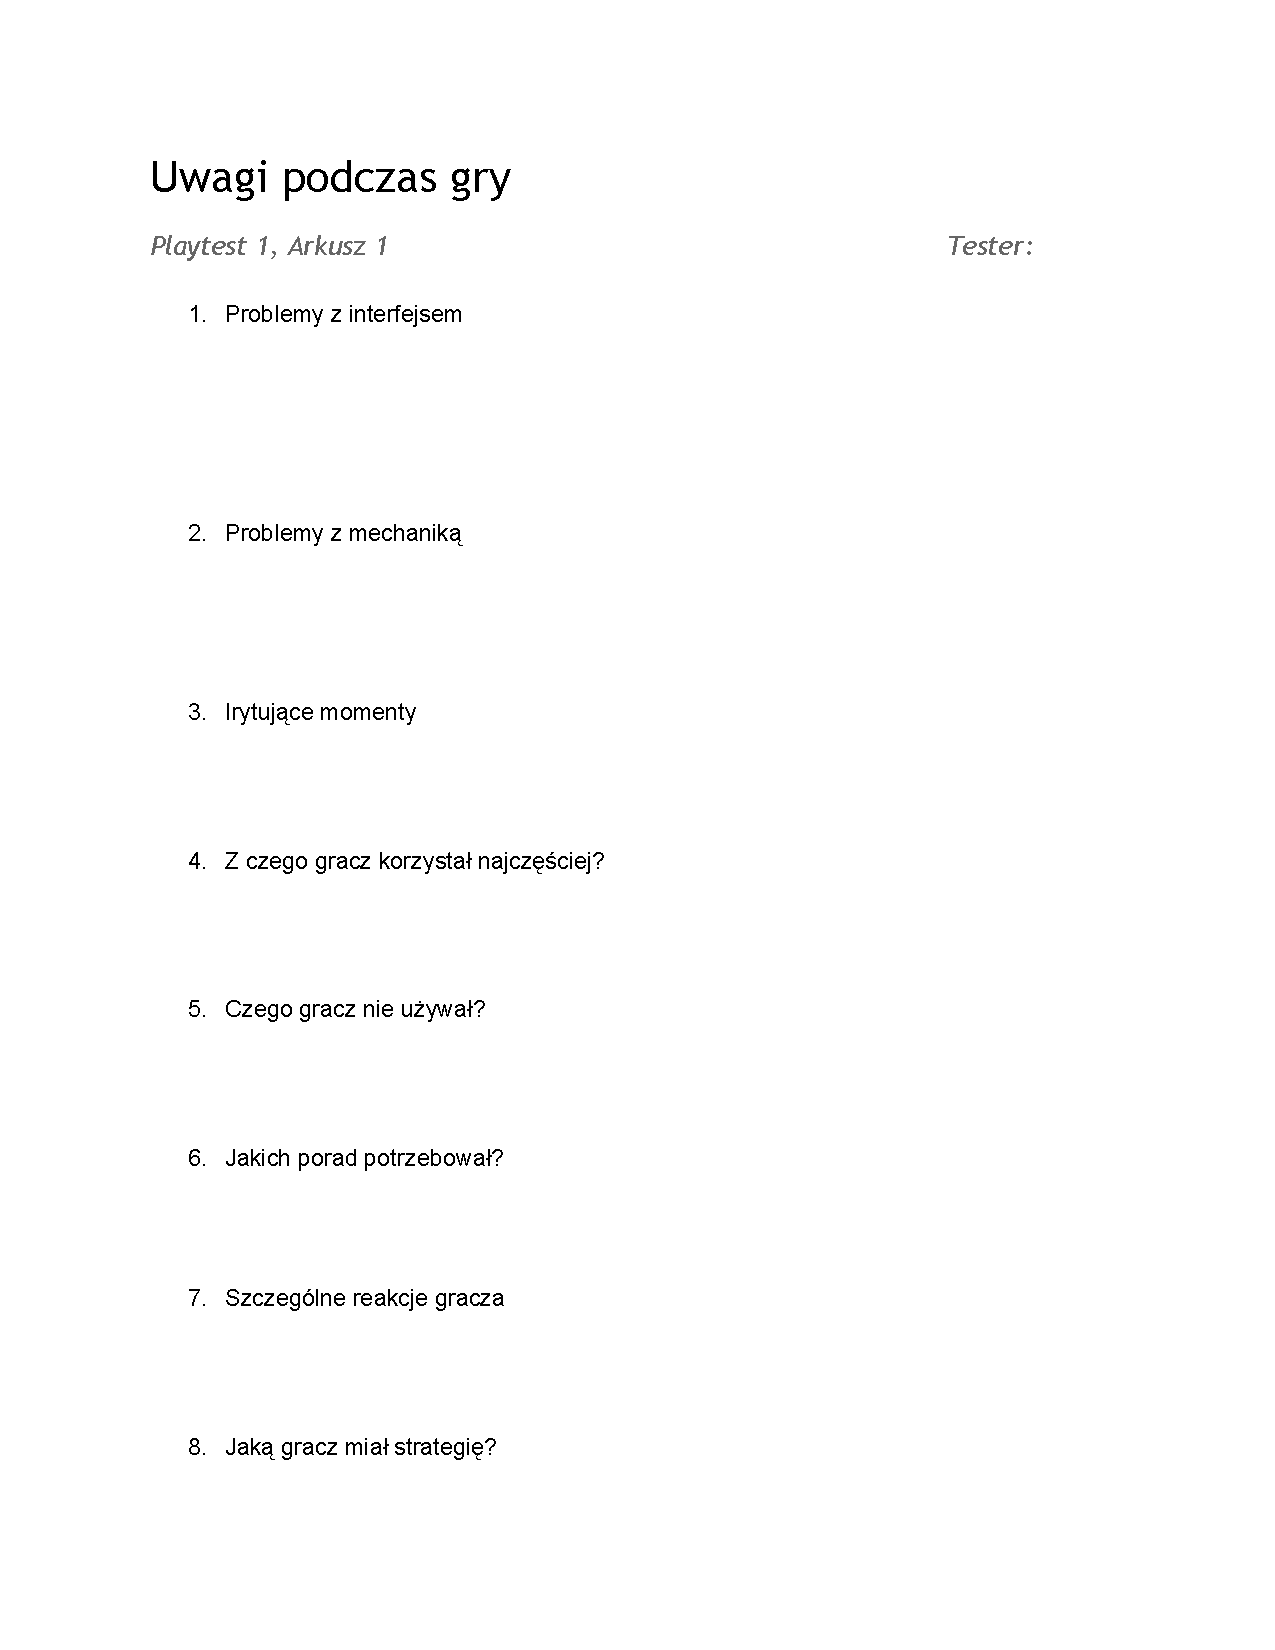
\includepdf[pages={-}]{Formularze-playtesty.pdf}
   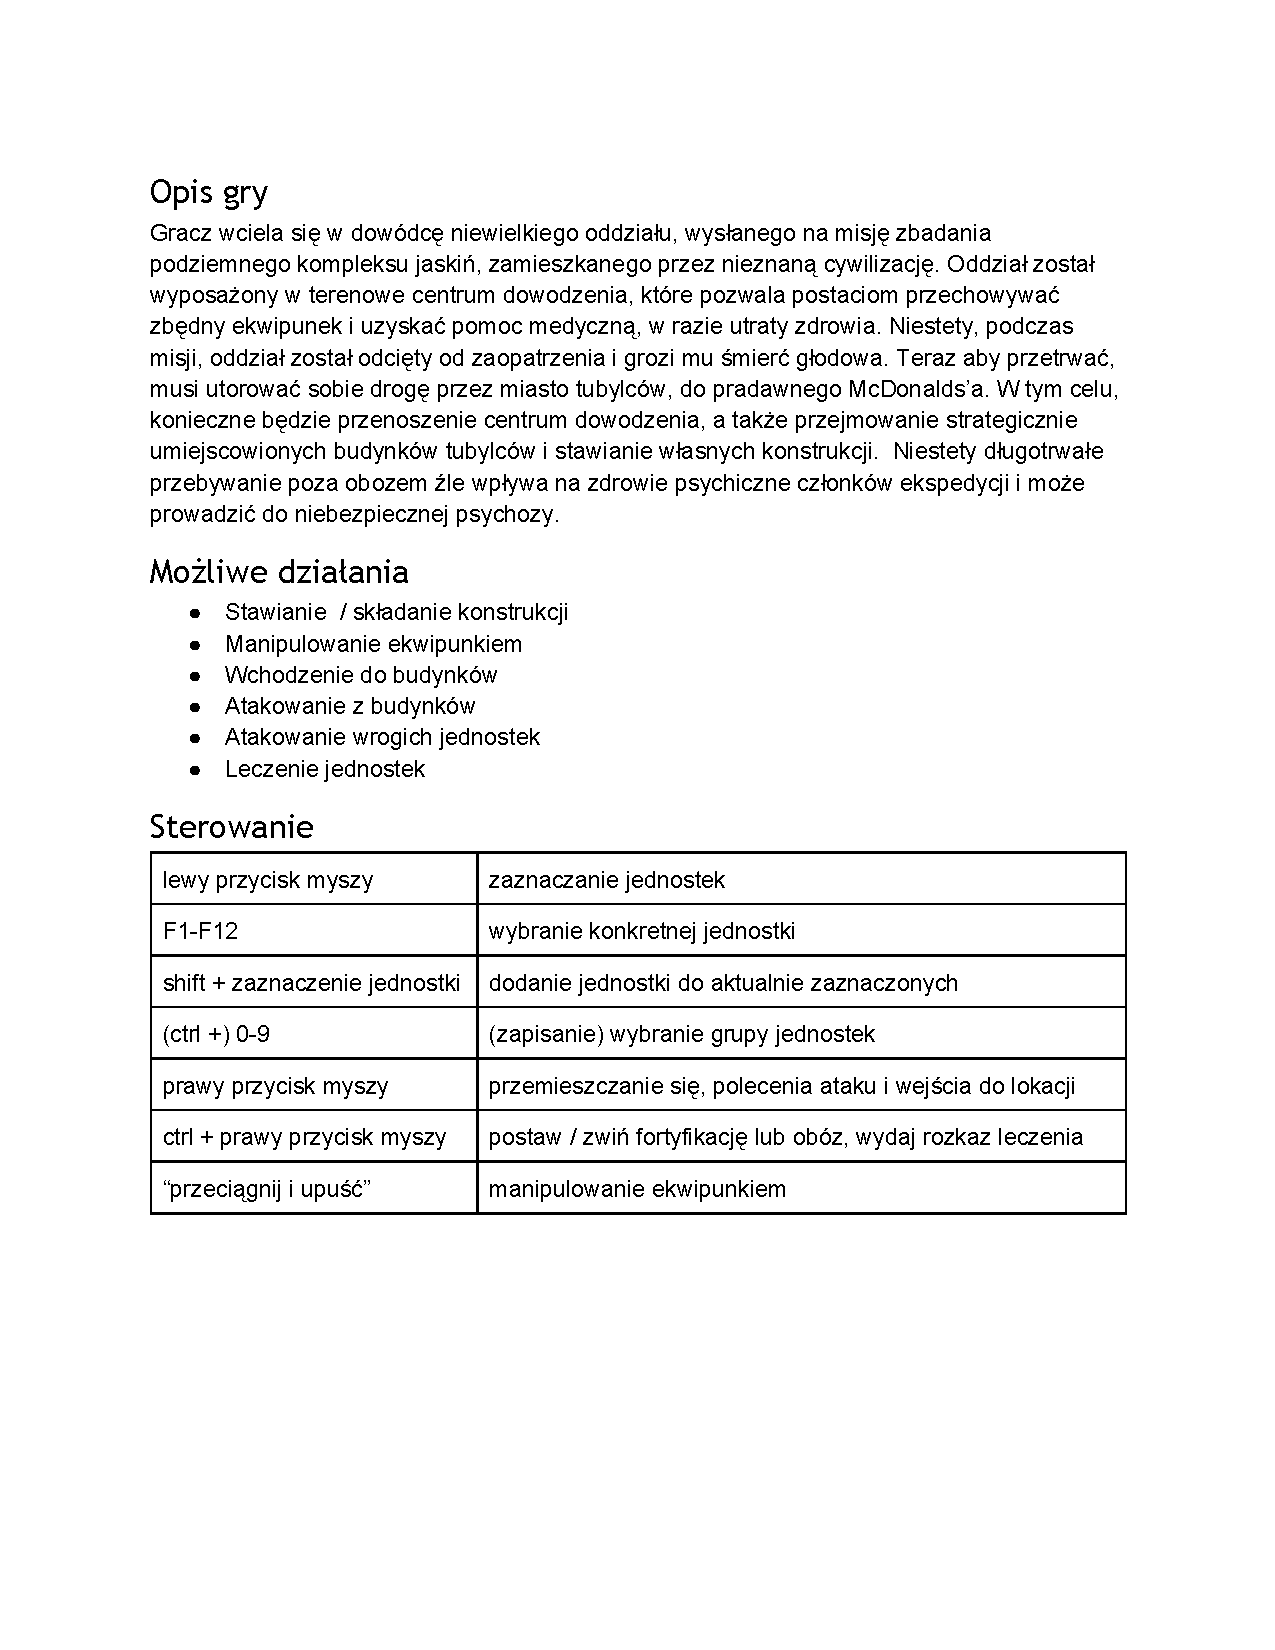
\includepdf[pages={-}]{Instrukcje-do-playtestow.pdf}
   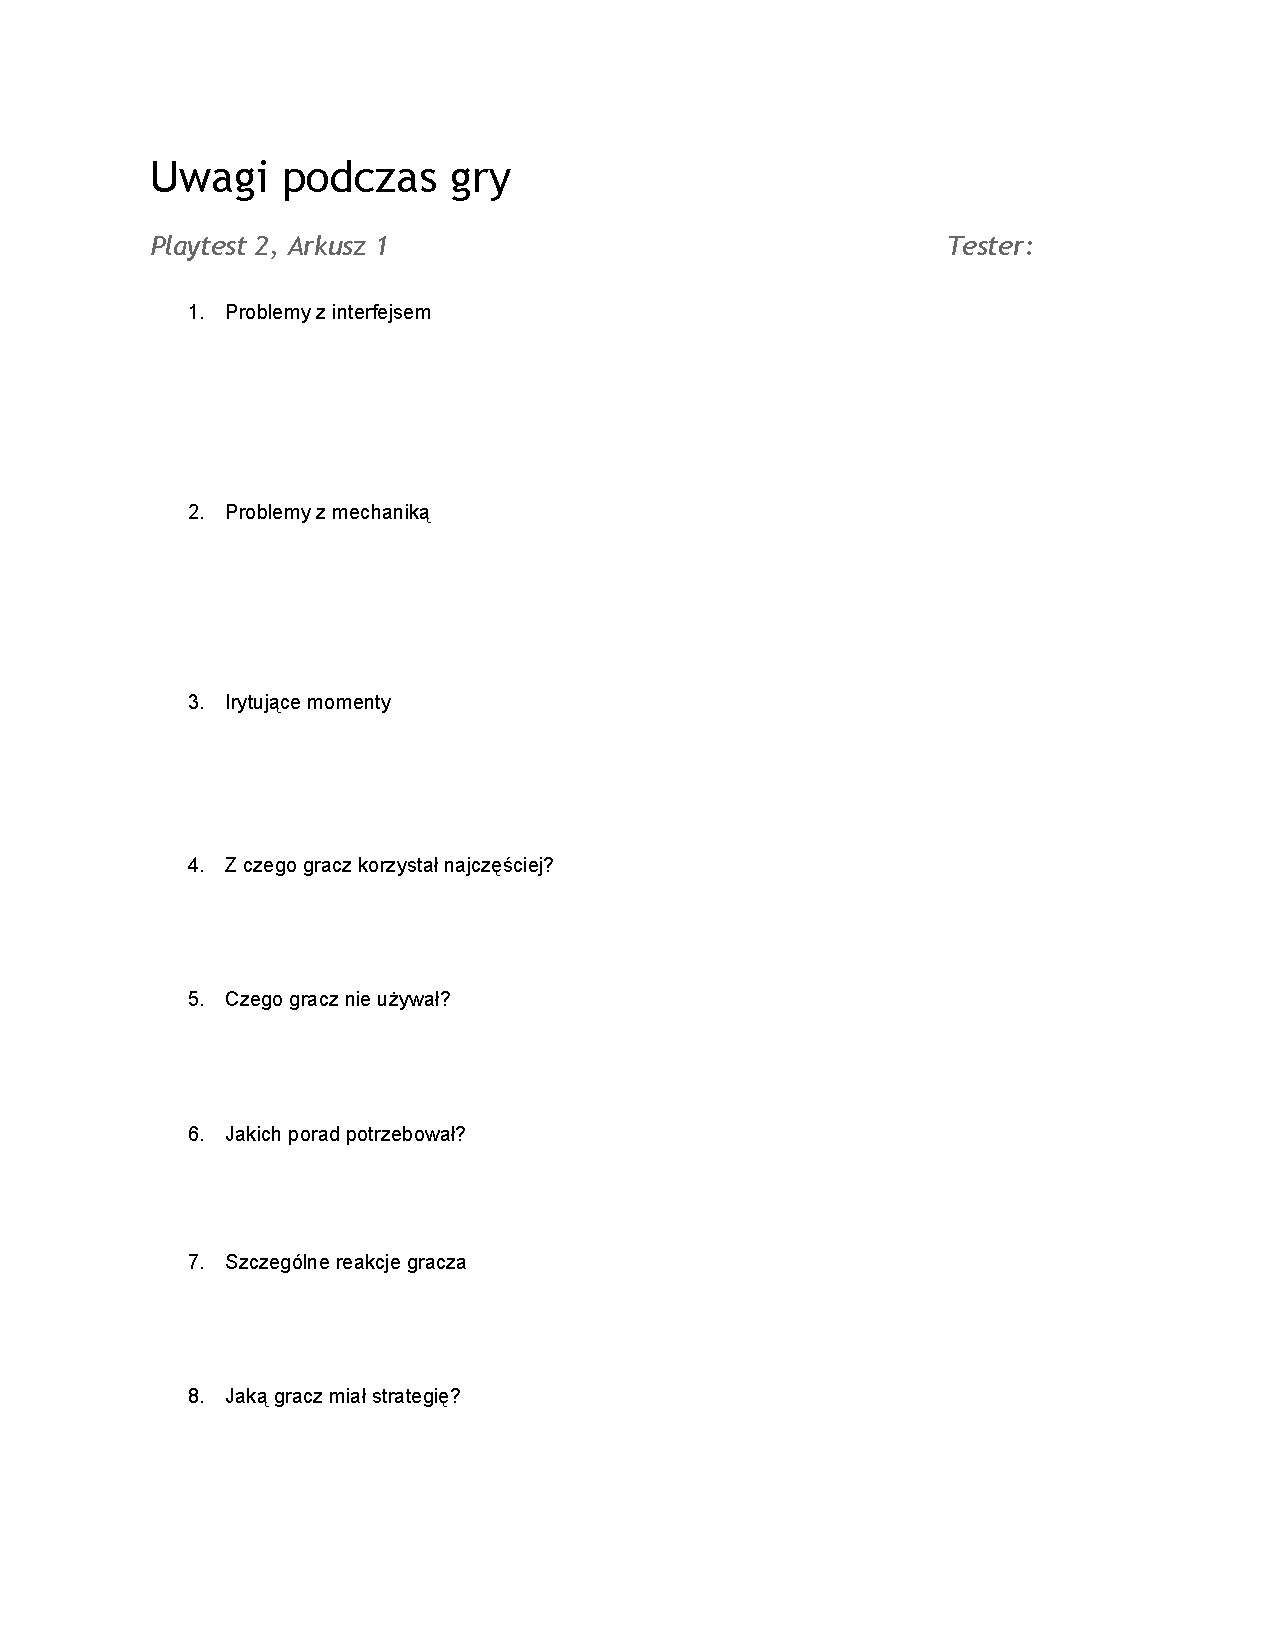
\includepdf[pages={-}]{Formularze-playtesty2.pdf}

\chapter{Zawarość płyty CD}
  Na płycie dostarczonej razem z~pracą licencjacką znajdują się:
  \begin{itemize}
   \item kod źródłowy gry \emph{Buried Secrets} wraz z~instrukcją instalacji w~katalogu z~kodem,
   \item pakiet RPM do instalacji programu w~systemie operacyjnym,
   \item dokumentacja techniczna programu,
   \item dokumenty pomocnicze opisujące wizję, założenia i~architekturę projektu,
   \item materiały wykorzystane do końcowej prezentacji projektu.
  \end{itemize}

\begin{thebibliography}{99}
  \addcontentsline{toc}{chapter}{Bibliografia}

  \bibitem{CA} \url{http://en.wikipedia.org/wiki/Video_game#Commercial_aspects}
  \bibitem{GB} \url{http://en.wikipedia.org/wiki/Gaussian_blur}
  \bibitem{A*} \url{http://en.wikipedia.org/wiki/A*_search_algorithm}
  \bibitem{HPA} BOTEA, Adi; MÜLLER, Martin; SCHAEFFER, Jonathan. Near optimal hierarchical path-finding. Journal of game development, 2004, 1.1: 7-28.
  \bibitem{QT} Dokumentacja techniczna Qt, \url{http://doc.qt.io/qt-5/reference-overview.html}
  \bibitem{SFML} Dokumentacja techniczna SFML, \url{http://www.sfml-dev.org/documentation/2.3/}
  \bibitem{BOX} Dokumentacja techniczna Box2d, \url{http://box2d.org/documentation/}
  
  
\end{thebibliography}

\end{document}


%%% Local Variables:
%%% mode: latex
%%% TeX-master: t
%%% coding: utf8
%%% End:
